% Options for packages loaded elsewhere
% Options for packages loaded elsewhere
\PassOptionsToPackage{unicode}{hyperref}
\PassOptionsToPackage{hyphens}{url}
\PassOptionsToPackage{dvipsnames,svgnames,x11names}{xcolor}
%
\documentclass[
  brazilian,
  authoryear,
  preprint]{elsarticle}
\usepackage{xcolor}
\usepackage{amsmath,amssymb}
\setcounter{secnumdepth}{5}
\usepackage{iftex}
\ifPDFTeX
  \usepackage[T1]{fontenc}
  \usepackage[utf8]{inputenc}
  \usepackage{textcomp} % provide euro and other symbols
\else % if luatex or xetex
  \usepackage{unicode-math} % this also loads fontspec
  \defaultfontfeatures{Scale=MatchLowercase}
  \defaultfontfeatures[\rmfamily]{Ligatures=TeX,Scale=1}
\fi
\usepackage{lmodern}
\ifPDFTeX\else
  % xetex/luatex font selection
\fi
% Use upquote if available, for straight quotes in verbatim environments
\IfFileExists{upquote.sty}{\usepackage{upquote}}{}
\IfFileExists{microtype.sty}{% use microtype if available
  \usepackage[]{microtype}
  \UseMicrotypeSet[protrusion]{basicmath} % disable protrusion for tt fonts
}{}
\makeatletter
\@ifundefined{KOMAClassName}{% if non-KOMA class
  \IfFileExists{parskip.sty}{%
    \usepackage{parskip}
  }{% else
    \setlength{\parindent}{0pt}
    \setlength{\parskip}{6pt plus 2pt minus 1pt}}
}{% if KOMA class
  \KOMAoptions{parskip=half}}
\makeatother
% Make \paragraph and \subparagraph free-standing
\makeatletter
\ifx\paragraph\undefined\else
  \let\oldparagraph\paragraph
  \renewcommand{\paragraph}{
    \@ifstar
      \xxxParagraphStar
      \xxxParagraphNoStar
  }
  \newcommand{\xxxParagraphStar}[1]{\oldparagraph*{#1}\mbox{}}
  \newcommand{\xxxParagraphNoStar}[1]{\oldparagraph{#1}\mbox{}}
\fi
\ifx\subparagraph\undefined\else
  \let\oldsubparagraph\subparagraph
  \renewcommand{\subparagraph}{
    \@ifstar
      \xxxSubParagraphStar
      \xxxSubParagraphNoStar
  }
  \newcommand{\xxxSubParagraphStar}[1]{\oldsubparagraph*{#1}\mbox{}}
  \newcommand{\xxxSubParagraphNoStar}[1]{\oldsubparagraph{#1}\mbox{}}
\fi
\makeatother


\usepackage{longtable,booktabs,array}
\usepackage{calc} % for calculating minipage widths
% Correct order of tables after \paragraph or \subparagraph
\usepackage{etoolbox}
\makeatletter
\patchcmd\longtable{\par}{\if@noskipsec\mbox{}\fi\par}{}{}
\makeatother
% Allow footnotes in longtable head/foot
\IfFileExists{footnotehyper.sty}{\usepackage{footnotehyper}}{\usepackage{footnote}}
\makesavenoteenv{longtable}
\usepackage{graphicx}
\makeatletter
\newsavebox\pandoc@box
\newcommand*\pandocbounded[1]{% scales image to fit in text height/width
  \sbox\pandoc@box{#1}%
  \Gscale@div\@tempa{\textheight}{\dimexpr\ht\pandoc@box+\dp\pandoc@box\relax}%
  \Gscale@div\@tempb{\linewidth}{\wd\pandoc@box}%
  \ifdim\@tempb\p@<\@tempa\p@\let\@tempa\@tempb\fi% select the smaller of both
  \ifdim\@tempa\p@<\p@\scalebox{\@tempa}{\usebox\pandoc@box}%
  \else\usebox{\pandoc@box}%
  \fi%
}
% Set default figure placement to htbp
\def\fps@figure{htbp}
\makeatother



\ifLuaTeX
\usepackage[bidi=basic]{babel}
\else
\usepackage[bidi=default]{babel}
\fi
% get rid of language-specific shorthands (see #6817):
\let\LanguageShortHands\languageshorthands
\def\languageshorthands#1{}


\setlength{\emergencystretch}{3em} % prevent overfull lines

\providecommand{\tightlist}{%
  \setlength{\itemsep}{0pt}\setlength{\parskip}{0pt}}



 
\usepackage[]{natbib}
\bibliographystyle{elsarticle-harv}


\usepackage{xcolor}
\usepackage{float}
\makeatletter
\@ifpackageloaded{caption}{}{\usepackage{caption}}
\AtBeginDocument{%
\ifdefined\contentsname
  \renewcommand*\contentsname{Índice}
\else
  \newcommand\contentsname{Índice}
\fi
\ifdefined\listfigurename
  \renewcommand*\listfigurename{Lista de Figuras}
\else
  \newcommand\listfigurename{Lista de Figuras}
\fi
\ifdefined\listtablename
  \renewcommand*\listtablename{Lista de Tabelas}
\else
  \newcommand\listtablename{Lista de Tabelas}
\fi
\ifdefined\figurename
  \renewcommand*\figurename{Figura}
\else
  \newcommand\figurename{Figura}
\fi
\ifdefined\tablename
  \renewcommand*\tablename{Tabela}
\else
  \newcommand\tablename{Tabela}
\fi
}
\@ifpackageloaded{float}{}{\usepackage{float}}
\floatstyle{ruled}
\@ifundefined{c@chapter}{\newfloat{codelisting}{h}{lop}}{\newfloat{codelisting}{h}{lop}[chapter]}
\floatname{codelisting}{Listagem}
\newcommand*\listoflistings{\listof{codelisting}{Lista de Listagens}}
\makeatother
\makeatletter
\makeatother
\makeatletter
\@ifpackageloaded{caption}{}{\usepackage{caption}}
\@ifpackageloaded{subcaption}{}{\usepackage{subcaption}}
\makeatother
\journal{Catena}
\usepackage{bookmark}
\IfFileExists{xurl.sty}{\usepackage{xurl}}{} % add URL line breaks if available
\urlstyle{same}
\hypersetup{
  pdftitle={Impedância hidráulica e vulnerabilidade geotécnica como amplificadores da erodibilidade efetiva em Plintossolos tropicais com erosão linear},
  pdfauthor={Luiz Diego Vidal Santos},
  pdflang={pt-BR},
  pdfkeywords={USLE correction factor, iron cementation, dispersible
fraction, jet erosion test, hierarchical Bayesian calibration},
  colorlinks=true,
  linkcolor={blue},
  filecolor={Maroon},
  citecolor={Blue},
  urlcolor={Blue},
  pdfcreator={LaTeX via pandoc}}


\setlength{\parindent}{6pt}
\begin{document}

\begin{frontmatter}
\title{Impedância hidráulica e vulnerabilidade geotécnica como
amplificadores da erodibilidade efetiva em Plintossolos tropicais com
erosão linear}
\author[1]{Luiz Diego Vidal Santos%
\corref{cor1}%
}
 \ead{ldvsantos@uefs.br} 

\affiliation[1]{organization={Universidade Estadual de Feira de
Santana, DCHF},city={Feira de
Santana},country={Brasil},countrysep={,},postcodesep={}}

\cortext[cor1]{Corresponding author}

        
\begin{abstract}
A erosão hídrica em vertentes tropicais com escoamento concentrado ativo
pode produzir respostas hidrossedimentológicas que a USLE/RUSLE,
concebida para erosão laminar e em sulcos, tende a representar apenas
parcialmente. Nessas condições, o fator de erodibilidade (\(K\))
estimado pelo nomograma de Wischmeier pode não captar plenamente
impedância hidráulica subsuperficial, toxicidade edáfica por alumínio e
vulnerabilidade geotécnica ao colapso de taludes, mecanismos
potencialmente relevantes em Plintossolos tropicais e capazes de afetar
a quantificação da carga sólida e o dimensionamento de medidas de
controle hidrossedimentológico. Este estudo avalia se a convergência de
impedância hidráulica subsuperficial, toxicidade edáfica por alumínio e
vulnerabilidade geotécnica ao colapso de taludes pode amplificar a
erodibilidade efetiva de Plintossolos tropicais além do previsto pelo
nomograma de Wischmeier, por meio de um fator de correção multiplicativo
(\(K_{plint}\)) calibrado experimentalmente em parcelas de campo. A
formulação adota
\(K_{plint} = K_{RUSLE} \times \alpha \times \beta \times \gamma\), em
que \(\alpha\) expressa amplificação por regime hidráulico, \(\beta\)
representa penalização por toxicidade edáfica e \(\gamma\) quantifica a
contribuição geotécnica associada à razão \(H/H_c\). O modelo
mecanístico de dispersão baseado em fração de ferro livre, densidade
aparente e hidrofobicidade pós-secagem opera como base auxiliar para
interpretar fisicamente a discrepância entre erodibilidade aparente e
efetiva e para condicionar a validação laboratorial da proposta. O
desenho experimental distribuirá 14 parcelas Wischmeier e microparcelas
com disdrômetro a laser em três sítios contrastantes, com Plintossolo
como alvo de calibração, Latossolo como controle negativo e Argissolo
como controle parcial, além de incorporar chuva simulada, Jet Erosion
Test invertido, microtomografia de raios X e fotogrametria dronada
bimestral para rastrear a evolução morfológica das feições. A estimação
combinará mínimos quadrados não lineares e modelagem hierárquica
bayesiana, usando intensidade de pico e energia cinética da chuva como
preditores hierárquicos para reduzir extrapolação para regimes
pluviométricos não observados. Cinco testes computacionais prévios
sugerem viabilidade matemática e consistência física da formulação,
indicando que o protocolo pode fornecer um fator de correção com
interpretabilidade física e potencial de transferência para Plintossolos
de outras regiões fisiográficas tropicais.
\end{abstract}





\begin{keyword}
    USLE correction factor \sep iron cementation \sep dispersible
fraction \sep jet erosion test \sep 
    hierarchical Bayesian calibration
\end{keyword}
\end{frontmatter}
    

\section{Introdução}\label{introduuxe7uxe3o}

Em solos tropicais, a erosão hídrica acelerada constitui uma das
principais ameaças à sustentabilidade, com taxas de perda que excedem a
pedogênese natural em ordens de grandeza nas vertentes mais vulneráveis
\citep{poesen_2018}. A Equação Universal de Perdas de Solo (USLE), na
formulação original de \citet{wischmeier_smith_1978} e na revisão RUSLE
de \citet{renard_et_al_1997}, permanece como o modelo empírico mais
adotado globalmente para estimativa de erosão laminar e em sulcos,
estruturando a perda de solo como produto de seis fatores que descrevem
erosividade da chuva, erodibilidade do solo, comprimento e declividade
da rampa, cobertura vegetal e práticas conservacionistas.

Na USLE/RUSLE, o fator de erodibilidade (\(K\)) sintetiza a
suscetibilidade intrínseca do solo ao destacamento e transporte por
impacto de gotas e escoamento laminar. Sua estimativa pelo nomograma de
\citet{wischmeier_et_al_1971} depende de cinco propriedades do horizonte
superficial, notadamente granulometria, matéria orgânica, estrutura e
permeabilidade, e foi calibrada em parcelas experimentais de solos
temperados do Meio-Oeste dos Estados Unidos, em condições edáficas e
climáticas distintas dos trópicos úmidos \citep{alewell_et_al_2019}. A
aplicação desse nomograma a solos tropicais intemperizados enfrenta
limitações reconhecidas na literatura.

Solos com elevada fração argilosa (\textgreater{} 40\%) mas com argilas
1:1 (caulinita) e oxi-hidróxidos de ferro e alumínio apresentam
microagregação estável que reduz a erodibilidade efetiva em relação ao
previsto pela granulometria
\citep{silva_et_al_2009, bertoni_lombardi_neto_2017}, ao passo que em
Plintossolos com impedância hidráulica em subsuperfície a erodibilidade
efetiva pode superar a prevista porque a geração de escoamento
concentrado sob intensidades de chuva recorrentes amplifica o
destacamento em magnitudes que a equação empírica não prevê
\citep{poesen_2018, cassol_et_al_2023}.

Essa discrepância é particularmente aguda quando a erosão transcende o
domínio laminar e em sulcos para o qual a USLE foi calibrada. Em
vertentes com ravinas ativas, a perda de solo integra contribuições de
incisão vertical, colapso de taludes e recuo de cabeceira, processos
governados por tensão cisalhante do escoamento concentrado e por
resistência geotécnica do substrato (coesão, ângulo de atrito, pressões
neutras) que o fator \(K\) não contempla
\citep{poesen_et_al_2003, liu_et_al_2021}. Modelos como EGEM, WEPP e
SWAT tratam erosão em ravinas como processo separado, porém sua
complexidade computacional e demanda de dados limitam a adoção em
contextos operacionais de planejamento \citep{alewell_et_al_2019}.

Três condições edáficas podem convergir em Plintossolos tropicais para
amplificar a erodibilidade efetiva de modo não captado pelo nomograma
\citep{padmanabhan_2005, ribeiro_filho_et_al_2023}. A impedância
hidráulica associada à presença de plintita em subsuperfície pode
reduzir substancialmente a velocidade de infiltração básica (VIB) e
favorecer a transição do regime de percolação vertical para escoamento
hortoniano quando a intensidade da chuva excede a capacidade de
infiltração do perfil
\citep{padmanabhan_2005, wang_et_al_2020, horton_1933}. A saturação por
alumínio elevada nos horizontes subsuperficiais pode restringir a
colonização radicular e reduzir a cobertura vegetal, expondo o horizonte
a destacamento direto e retroalimentando a amplificação da erodibilidade
\citep{rao_et_al_2016, vannoppen_2015}. A proximidade geotécnica ao
limiar de ruptura por cisalhamento, expressa pela razão entre
profundidade da feição e altura crítica de Rankine (\(H/H_c\)), introduz
contribuição de colapso de taludes que cresce de modo não linear à
medida que a feição se aprofunda
\citep{poesen_et_al_2003, sidorchuk_2006}.

Nos Tabuleiros Costeiros de Sergipe, trabalho anterior caracterizou um
Plintossolo Argilúvico Distrófico com VIB de 1,53 cm/h nos terços
intermediário e inferior da vertente, saturação por alumínio de 84--99\%
nos horizontes subsuperficiais, coesão sob saturação de 13,02 kPa e
ângulo de atrito de 34,93° (horizonte Bt, 1,20 m), resultando em altura
crítica de corte vertical \(H_c\) = 3,35 m. Seis feições erosivas com
profundidade de 0,40--1,50 m e razão \(H/H_c\) de 0,12--0,45 foram
classificadas por inferência fuzzy Mamdani como ravinas transicionais a
voçorocas incipientes. Esses dados sugerem que a convergência das três
condições amplificadoras eleva a erodibilidade efetiva do Plintossolo
acima do previsto pelo nomograma, motivando a proposição de um fator de
correção específico.

Para verificar se essa amplificação é atribuível às propriedades
diagnósticas do Plintossolo, e não a um artefato generalizável a
qualquer solo tropical intemperizado, torna-se necessário o confronto
com classes pedológicas contrastantes. Latossolos Vermelho-Amarelos da
mesma região apresentam VIB tipicamente superior a 6 cm/h, saturação por
alumínio inferior a 30\% e feições erosivas lineares ausentes ou
incipientes, constituindo controle negativo no qual se espera
erodibilidade observada próxima à prevista pelo nomograma
\citep{silva_et_al_2009, bertoni_lombardi_neto_2017}. Argissolos
Vermelho-Amarelos, por sua vez, compartilham com o Plintossolo o
gradiente textural abrupto (horizonte Bt adensado) que gera impedância
hidráulica e redução da VIB, porém sem plintita e frequentemente com
saturação por alumínio intermediária, operando como controle parcial que
permite isolar o efeito do regime hidráulico das demais amplificações.

Até o presente momento, nenhum estudo propôs um fator de correção para o
\(K\) da USLE/RUSLE que incorpore simultaneamente impedância hidráulica
subsuperficial, toxicidade edáfica por alumínio e vulnerabilidade
geotécnica ao colapso de taludes, nem validou tal formulação por
confrontação multi-classe entre solos tropicais com gradientes
contrastantes dessas propriedades. A literatura tampouco derivou a
erodibilidade de Plintossolos a partir de princípios mecânicos do solo
cimentado por óxidos de ferro, limitando-se a correções empíricas do
nomograma que não captam a coesão adicional proveniente da cimentação
ferruginosa, a qual altera simultaneamente a agregação primária e a
condutividade hidráulica, tornando a resistência ao cisalhamento úmido
insatisfatoriamente representada por texturas-padrão
\citep{alewell_et_al_2019}. A ausência de um modelo mecanístico de
dispersão que integre fração de ferro livre, densidade aparente e
hidrofobicidade pós-secagem para predizer a fração dispersável sob chuva
impede a distinção entre erodibilidade aparente (captada pelo nomograma)
e erodibilidade efetiva (condicionada pela resposta do material
cimentado a ciclos de umedecimento e secagem).

Partindo desse quadro, este estudo propõe a fundamentação teórica e o
desenho experimental multi-classe para calibração de um fator de
correção multiplicativo (\(K_{plint}\)) que incorpora regime hidráulico,
toxicidade edáfica e vulnerabilidade geotécnica ao fator \(K\) da
USLE/RUSLE.

A formulação operacional em campo permanece restrita a esses três
amplificadores, enquanto o modelo mecanístico de dispersão atua como
submodelo auxiliar para quantificar, em laboratório, a discrepância
entre a fração textural fina e a fração efetivamente mobilizável do
material cimentado. O Plintossolo opera como alvo de calibração, o
Latossolo como controle negativo e o Argissolo como controle parcial,
configurando uma cadeia causal que preserva interpretabilidade física e
permite separar a contribuição de cada mecanismo amplificador. A
viabilidade matemática (identificabilidade paramétrica, sensibilidade e
consistência física) da formulação proposta foi previamente avaliada por
cinco testes computacionais apresentados em manuscrito complementar,
cujos resultados sustentam a adequação do desenho experimental aqui
descrito.

\section{Fundamentação teórica}\label{fundamentauxe7uxe3o-teuxf3rica}

\subsection{A USLE e o nomograma de
erodibilidade}\label{a-usle-e-o-nomograma-de-erodibilidade}

Na USLE, a perda de solo média anual é expressa como produto de seis
fatores (Equação~\ref{eq-usle}).

\begin{equation}\phantomsection\label{eq-usle}{
A = R \times K \times L \times S \times C \times P
}\end{equation}

onde \(A\) é a perda de solo média anual (t ha\(^{-1}\) ano\(^{-1}\)),
\(R\) o fator de erosividade da chuva (MJ mm ha\(^{-1}\) h\(^{-1}\)
ano\(^{-1}\)), \(K\) o fator de erodibilidade do solo (t h MJ\(^{-1}\)
mm\(^{-1}\)), \(L\) o fator de comprimento de rampa, \(S\) o fator de
declividade, \(C\) o fator de cobertura e manejo e \(P\) o fator de
práticas conservacionistas. O fator \(K\) é estimado pela equação do
nomograma (Equação~\ref{eq-nomograma}).

\begin{equation}\phantomsection\label{eq-nomograma}{
100\,K = 2{,}1 \times 10^{-4}\,M^{1{,}14}\,(12 - a) + 3{,}25\,(b - 2) + 2{,}5\,(c - 3)
}\end{equation}

onde
\(M = (\%\text{silte} + \%\text{areia muito fina}) \times (100 - \%\text{argila})\),
\(a\) é o teor de matéria orgânica (\%), \(b\) o código de estrutura do
solo (1--4) e \(c\) o código de permeabilidade (1--6).

\subsection{Modelo mecanístico de dispersão em solos cimentados por
óxidos de
ferro}\label{modelo-mecanuxedstico-de-dispersuxe3o-em-solos-cimentados-por-uxf3xidos-de-ferro}

Na calibração convencional do fator \(K\), a regressão direta contra
perda de solo total trata a erodibilidade como propriedade escalar
determinada por granulometria e matéria orgânica, sem representar o
mecanismo pelo qual o material edáfico é efetivamente mobilizado sob
ação da chuva. Em Plintossolos, a cimentação parcial por oxi-hidróxidos
de ferro (goethita e hematita) confere coesão adicional à matriz que não
é captada pelo nomograma, pois este assume que a fração dispersável
coincide com a fração textural fina \citep{alewell_et_al_2019}.

A pseudoplenitação altera simultaneamente a agregação primária, pela
formação de pontes de óxidos entre domínios cauliníticos, e a
condutividade hidráulica, pela obstrução parcial de macroporos com
material ferruginoso precipitado, de modo que a resistência ao
cisalhamento úmido do agregado cimentado excede substancialmente a do
mesmo material desferrificado \citep{silva_et_al_2009}.

Neste estudo, a abordagem mecanística substitui a regressão direta por
uma cadeia causal em duas etapas. Na primeira, estima-se a fração
dispersável (\(f_d\)) a partir de um modelo de mistura que integra a
fração de ferro livre extraída por ditionito-citrato-bicarbonato
(\(Fe_d\), g kg\(^{-1}\)), a densidade aparente (\(\rho_b\), g
cm\(^{-3}\)) e o índice de hidrofobicidade pós-secagem (\(R_{WDPT}\),
tempo de penetração da gota em segundos) como variáveis preditoras da
proporção do solo efetivamente suscetível à desagregação sob impacto de
gotas e escoamento raso (Equação~\ref{eq-fd}).

\begin{equation}\phantomsection\label{eq-fd}{
f_d = \dfrac{f_{tex}}{1 + a_1 \cdot Fe_d^{a_2} \cdot \rho_b^{a_3} \cdot R_{WDPT}^{a_4}}
}\end{equation}

onde \(f_{tex}\) é a fração dispersável teórica calculada pela
granulometria convencional (equivalente ao parâmetro \(M\) do nomograma)
e os coeficientes \(a_1\)--\(a_4\) são parâmetros a calibrar
experimentalmente por ensaios de dispersão sob chuva simulada em
amostras com teores contrastantes de ferro livre. A forma funcional
assegura que \(f_d \to f_{tex}\) quando a cimentação por ferro é
desprezível (\(Fe_d \to 0\)) e \(f_d \to 0\) quando a cimentação é
extrema, comportamento fisicamente coerente com a estabilização
progressiva de microagregados por pontes de óxidos
\citep{bertoni_lombardi_neto_2017}.

Na segunda etapa, a fração dispersável estimada pela Equação~\ref{eq-fd}
é propagada para o cálculo da energia de desagregação específica
(\(E_d\), J kg\(^{-1}\)), definida como a energia cinética de chuva
necessária para mobilizar uma unidade de massa do material cimentado em
relação ao material desferrificado (Equação~\ref{eq-ed}).

\begin{equation}\phantomsection\label{eq-ed}{
E_d = E_0 \cdot \left(\dfrac{f_{tex}}{f_d}\right)^{n_d}
}\end{equation}

onde \(E_0\) é a energia de desagregação de referência para o solo
desferrificado (calibrada em laboratório por chuva simulada sobre
amostra tratada com ditionito) e \(n_d\) o expoente de resistência à
desagregação. A razão \(f_{tex}/f_d > 1\) indica que a cimentação por
ferro eleva a energia necessária para destacar partículas em relação ao
previsto pela textura, quantificando a discrepância mecanística que o
nomograma ignora. Nesta proposta, \(E_d\) não constitui um quarto fator
explícito do \(K_{plint}\), mas uma variável mecanística auxiliar usada
para verificar se a cimentação ferruginosa altera a resistência
intrínseca ao destacamento na mesma direção observada na resposta
hidrológica e na erodibilidade medida em campo.

Experimentalmente, a validação do modelo de mistura requer ensaios de
dispersão sob chuva simulada em amostras naturais e desferrificadas do
mesmo horizonte, conforme descrito na seção 5.4, permitindo estimar
\(a_1\)--\(a_4\) e \(n_d\) independentemente dos parâmetros do fator de
correção (\(n_1\), \(\beta_{max}\), \(k_2\), \(k_3\), \(n_3\)). Essa
separação aloca o modelo de dispersão no nível laboratorial da cadeia
causal, ao passo que os termos \(\alpha\), \(\beta\) e \(\gamma\)
permanecem como amplificadores operacionais calibrados em parcela,
evitando a colinearidade que compromete regressões diretas com muitos
preditores simultâneos.

\subsection{\texorpdfstring{Estrutura do fator de correção
\(K_{plint}\)}{Estrutura do fator de correção K\_\{plint\}}}\label{estrutura-do-fator-de-correuxe7uxe3o-k_plint}

O modelo mecanístico apresentado na seção anterior não introduz um
quarto fator multiplicativo, mas fornece a base laboratorial para
interpretar fisicamente a amplificação estimada em campo. Assim, para
Plintossolos tropicais com erosão linear, a erodibilidade corrigida é
expressa como produto do fator \(K\) do nomograma de Wischmeier por três
termos de correção adimensionais (Equação~\ref{eq-kplint}). A fração
dispersável e a energia de desagregação derivadas da Equação~\ref{eq-fd}
e da Equação~\ref{eq-ed} funcionam como variáveis auxiliares de
condicionamento e validação, enquanto a correção operacional permanece
restrita aos três mecanismos observáveis em escala de parcela.

\begin{equation}\phantomsection\label{eq-kplint}{
K_{plint} = K_{RUSLE} \times \alpha(VIB) \times \beta(m_{Al}) \times \gamma\!\left(\dfrac{H}{H_c}\right)
}\end{equation}

onde \(K_{RUSLE}\) é o fator de erodibilidade obtido pela
Equação~\ref{eq-nomograma} ou por medição direta em parcela padrão,
\(\alpha\) o fator de amplificação por regime hidráulico, \(\beta\) o
fator de penalização por toxicidade edáfica e \(\gamma\) o fator de
vulnerabilidade geotécnica. A estrutura multiplicativa implica que cada
fator opera como amplificador independente.

Quando nenhuma das três condições amplificadoras está presente (solo bem
drenado, ausência de toxicidade por alumínio, ausência de feição erosiva
profunda), os três fatores assumem valor unitário e \(K_{plint}\) se
reduz a \(K_{RUSLE}\). Quando as três condições convergem, como em
Plintossolos com voçorocas ativas, os fatores se multiplicam e a razão
\(\delta = K_{plint}/K_{RUSLE} = \alpha \times \beta \times \gamma\)
pode atingir valores de 2 a 10 ou superiores \citep{poesen_2018}. A
variável \(\delta\) é adimensional e independente do valor absoluto de
\(K_{RUSLE}\), permitindo comparar o grau de amplificação entre classes
pedológicas com erodibilidade basal distinta.

\subsection{\texorpdfstring{Fator de amplificação por regime hidráulico
\(\alpha(VIB)\)}{Fator de amplificação por regime hidráulico \textbackslash alpha(VIB)}}\label{fator-de-amplificauxe7uxe3o-por-regime-hidruxe1ulico-alphavib}

No nomograma de Wischmeier, a permeabilidade recebe peso relativamente
baixo no cômputo de \(K\) (código 1--6, contribuição máxima de 7,5\% no
valor final). Em solos com boa drenagem interna, a maior parte da
precipitação infiltra e percola verticalmente, gerando pouco escoamento
superficial e, consequentemente, baixa energia disponível para
destacamento e transporte de partículas \citep{deroo_1992}. Em
Plintossolos, horizontes subsuperficiais com plintita ou petroplintita
apresentam condutividade hidráulica saturada muito inferior à dos
horizontes sobrejacentes, criando barreira à percolação que favorece a
saturação do perfil e o escoamento hortoniano por excesso de saturação
\citep{padmanabhan_2005}. A VIB, determinada em campo por infiltrômetro
de duplo anel, reflete essa impedância integrada ao longo do perfil e
constitui a variável de entrada mais acessível para expressar o
contraste hidrológico entre classes de solo
\citep{bertoni_lombardi_neto_2017}.

No Plintossolo estudado, a VIB varia de 3,13 cm/h no terço superior a
1,53 cm/h no intermediário (redução de 51\%), transição que converte o
regime de percolação vertical predominante em escoamento hortoniano e
amplifica a energia erosiva efetiva de modo desproporcional ao previsto
pelo código de permeabilidade do nomograma \citep{poesen_2018}.

Como forma funcional para \(\alpha\), propõe-se uma lei de potência
referenciada a um limiar de VIB acima do qual o perfil opera
predominantemente sob regime de percolação vertical e a contribuição da
impedância hidráulica à erodibilidade é negligenciável
(Equação~\ref{eq-alpha}).

\begin{equation}\phantomsection\label{eq-alpha}{
\alpha(VIB) = \left(\dfrac{VIB_{ref}}{VIB_{local}}\right)^{n_1}
}\end{equation}

onde \(VIB_{ref}\) é o limiar de referência (cm/h) acima do qual o
perfil opera sob percolação vertical predominante e \(n_1\) o expoente
de amplificação a calibrar. O expoente \(n_1\) governa a intensidade da
penalização à medida que a VIB decresce, de modo que para \(n_1 = 1\) a
relação é linear e reduzir a VIB pela metade duplica \(\alpha\),
enquanto valores de \(n_1 > 1\) produzem penalização mais severa em
solos com impedância acentuada e \(n_1 < 1\) atenua a diferenciação
entre solos com VIB moderada e muito baixa \citep{kinnell_2005}. O
limiar \(VIB_{ref}\) = 6,0 cm/h corresponde ao limite inferior de solos
classificados como bem drenados na pedologia tropical
\citep{embrapa_2018} e foi adotado como ponto de neutralidade
(\(\alpha = 1\)) do fator hidráulico.

Esse valor foi corroborado empiricamente pela classificação fuzzy de
severidade desenvolvida para o sítio, na qual feições situadas acima
desse patamar não atingem severidade transicional mesmo com
profundidades de 2 m.

Para \(VIB_{local} \geq VIB_{ref}\), adota-se \(\alpha = 1\) (sem
correção). Para \(VIB_{local} < VIB_{ref}\), \(\alpha > 1\) com
magnitude crescente conforme o inverso da infiltração. No Plintossolo
estudado, a VIB do horizonte intermediário (BAc) é 1,53 cm/h, resultando
em \(\alpha = (6{,}0/1{,}53)^{n_1} = 3{,}92^{n_1}\), o que para
\(n_1 = 1\) indica que a impedância hidráulica subsuperficial amplifica
a erodibilidade efetiva em quase quatro vezes em relação a um solo com
VIB de referência. Um Latossolo Vermelho-Amarelo típico com VIB de 9
cm/h apresenta \(\alpha = 1\) (\(VIB > VIB_{ref}\)), ilustrando a
capacidade do fator de distinguir classes bem drenadas de classes com
impedância hidráulica sem modelagem hidrológica detalhada. Os valores de
\(\alpha\) para três posições da vertente e cenários de \(n_1\) são
apresentados na Tabela 1.

Tabela 1. Valores de \(\alpha\) para três posições da vertente em função
de \(n_1\) hipotético

\begin{longtable}[]{@{}
  >{\raggedright\arraybackslash}p{(\linewidth - 8\tabcolsep) * \real{0.1579}}
  >{\raggedleft\arraybackslash}p{(\linewidth - 8\tabcolsep) * \real{0.2105}}
  >{\raggedleft\arraybackslash}p{(\linewidth - 8\tabcolsep) * \real{0.2105}}
  >{\raggedleft\arraybackslash}p{(\linewidth - 8\tabcolsep) * \real{0.2105}}
  >{\raggedleft\arraybackslash}p{(\linewidth - 8\tabcolsep) * \real{0.2105}}@{}}
\toprule\noalign{}
\begin{minipage}[b]{\linewidth}\raggedright
Posição
\end{minipage} & \begin{minipage}[b]{\linewidth}\raggedleft
VIB (cm/h)
\end{minipage} & \begin{minipage}[b]{\linewidth}\raggedleft
\(\alpha\) (\(n_1\) = 0,5)
\end{minipage} & \begin{minipage}[b]{\linewidth}\raggedleft
\(\alpha\) (\(n_1\) = 1,0)
\end{minipage} & \begin{minipage}[b]{\linewidth}\raggedleft
\(\alpha\) (\(n_1\) = 1,5)
\end{minipage} \\
\midrule\noalign{}
\endhead
\bottomrule\noalign{}
\endlastfoot
Terço superior & 3,13 & 1,38 & 1,92 & 2,66 \\
Terço intermediário & 1,53 & 1,98 & 3,92 & 7,76 \\
Terço inferior & 1,59 & 1,94 & 3,77 & 7,33 \\
\end{longtable}

\subsection{\texorpdfstring{Fator de penalização por toxicidade edáfica
\(\beta(m_{Al})\)}{Fator de penalização por toxicidade edáfica \textbackslash beta(m\_\{Al\})}}\label{fator-de-penalizauxe7uxe3o-por-toxicidade-eduxe1fica-betam_al}

Nos horizontes subsuperficiais do Plintossolo estudado, a saturação por
alumínio (\(m\)) varia de 15,2\% no Ap a 99,2\% no BAc, constituindo
gradiente de toxicidade que restringe progressivamente a colonização
radicular e a cobertura vegetal \citep{de_oliveira_et_al_2024}.

Embora o fator \(C\) da USLE capture parcialmente o efeito da cobertura,
ele não incorpora o mecanismo causal edáfico que a determina nem a
retroalimentação entre perda de cobertura, exposição do horizonte e
amplificação da erodibilidade, processo cíclico documentado em solos
álicos tropicais \citep{cassol_et_al_2023}.

Como forma funcional, propõe-se uma sigmoide logística com inflexão no
limiar de caráter álico (Equação~\ref{eq-beta}).

\begin{equation}\phantomsection\label{eq-beta}{
\beta(m) = 1 + \dfrac{\beta_{max} - 1}{1 + \exp\!\left[-k_2\,(m - m_0)\right]}
}\end{equation}

onde \(m\) é a saturação por alumínio do horizonte diagnóstico (\%,
0--100), \(m_0\) o ponto de inflexão coincidente com o limiar
convencional de caráter álico (\%), \(k_2\) o parâmetro de inclinação da
sigmoide (adimensional) e \(\beta_{max}\) o fator máximo de
amplificação. Para \(m_{Al}\) muito abaixo de \(m_0\), o denominador é
grande e \(\beta\) se aproxima de 1, indicando que a fitotoxicidade é
insuficiente para suprimir mensuravelmente a vegetação. Para \(m_{Al}\)
muito acima de \(m_0\), a função converge para \(\beta_{max}\),
representando a amplificação máxima atribuível exclusivamente à
toxicidade. O parâmetro \(k_2\) controla a abruptidade da transição, com
valores altos produzindo mudança rápida em torno de 50\% e valores
baixos gerando gradiente suave ao longo de toda a faixa de saturação.

Com base na literatura de fitotoxicidade por alumínio em solos
tropicais, propõe-se \(m_0\) = 50\% como ponto de inflexão, valor acima
do qual a maioria das gramíneas forrageiras tropicais apresenta redução
de cobertura superior a 50\% \citep{embrapa_2018}. Os parâmetros \(k_2\)
e \(\beta_{max}\) constituem os termos a calibrar experimentalmente.
Para o Plintossolo estudado, considerando valores preliminares de
\(\beta_{max} = 2{,}5\) e \(k_2 = 0{,}10\), o horizonte Ap (\(m\) =
15,2\%) resulta em \(\beta \approx 1{,}04\), praticamente sem
amplificação, enquanto o horizonte BAc (\(m\) = 99,2\%) atinge
\(\beta \approx 2{,}47\), próximo ao máximo.

Agronomicamente, esse gradiente vertical indica que a superfície do solo
ainda pode sustentar cobertura vegetal esparsa, porém os horizontes
subsuperficiais expostos nos taludes das feições erosivas estão
desprovidos de proteção radicular contra o desprendimento por escoamento
concentrado \citep{vannoppen_2015}. A sigmoide captura essa não
linearidade com apenas dois parâmetros livres (\(\beta_{max}\) e
\(k_2\)).

\subsection{\texorpdfstring{Fator de vulnerabilidade geotécnica
\(\gamma(H/H_c)\)}{Fator de vulnerabilidade geotécnica \textbackslash gamma(H/H\_c)}}\label{fator-de-vulnerabilidade-geotuxe9cnica-gammahh_c}

Processos laminares e em sulcos orientaram a formulação original da
USLE, governada por destacamento superficial por impacto de gotas
(splash) e tensão cisalhante de escoamento raso. Em vertentes com
feições erosivas que se aprofundam em direção à altura crítica de
ruptura por cisalhamento (\(H_c\)), a contribuição de movimentos de
massa nas paredes das feições (escorregamentos translacionais e
rotacionais) à perda total de solo cresce de modo não linear, processo
que o fator \(K\) não contempla
\citep{poesen_et_al_2003, sidorchuk_2006}.

Como indicador adimensional normalizado da proximidade ao limiar de
ruptura, a razão \(H/H_c\) expressa a profundidade máxima da feição
dividida pela altura crítica de Rankine. Para \(H/H_c \to 0\) (sulcos
rasos), a contribuição geotécnica é desprezível; para \(H/H_c \to 1\), o
talude opera próximo ao equilíbrio limite e episódios de saturação
sazonal com desenvolvimento de poropressões positivas podem disparar
escorregamentos translacionais e mobilização volumétrica de solo,
amplificando a perda de solo em ordens de grandeza superiores ao
previsto pela USLE.

Como forma funcional, propõe-se uma função de potência com origem
unitária (Equação~\ref{eq-gamma}).

\begin{equation}\phantomsection\label{eq-gamma}{
\gamma\!\left(\dfrac{H}{H_c}\right) = 1 + k_3 \cdot \left(\dfrac{H}{H_c}\right)^{n_3}
}\end{equation}

onde \(H\) é a profundidade máxima da feição (m), \(H_c\) a altura
crítica de corte vertical sob saturação (m), \(k_3\) o coeficiente de
escala da amplificação geotécnica e \(n_3\) o expoente de curvatura da
resposta. Para \(H/H_c = 0\), \(\gamma = 1\) (sem contribuição
geotécnica).

Valores elevados de \(n_3\) (\textgreater{} 2) fazem com que \(\gamma\)
permaneça próximo de 1 para feições rasas e aumente abruptamente apenas
quando \(H/H_c\) se aproxima de 1, comportamento fisicamente coerente
porque o volume de solo mobilizado pela cunha de ruptura cresce com
potência cúbica ou superior da altura da parede. A escolha de
\(n_3 = 2\) como valor inicial é motivada pela dependência quadrática
entre volume mobilizado por colapso e altura de queda em modelos de
ruptura planar \citep{fredlund_rahardjo_1993}.

Pela teoria de Rankine para corte vertical com fissura de tração
preenchida por água, a altura crítica \(H_c\) é estimada por
(Equação~\ref{eq-hc}).

\begin{equation}\phantomsection\label{eq-hc}{
H_c = \dfrac{2\,c}{\gamma_{sat}} \cdot \tan\!\left(45° + \dfrac{\phi}{2}\right) + \dfrac{2\,c}{\gamma_{sat} \cdot \tan\!\left(45° + \dfrac{\phi}{2}\right)}
}\end{equation}

onde \(c\) é a coesão efetiva sob saturação (kPa), \(\phi\) o ângulo de
atrito interno (°) e \(\gamma_{sat}\) o peso específico saturado do solo
(kN/m³). A formulação assume análise em tensões totais com pressão
neutra nula (\(u = 0\)), consistente com a determinação de \(c\) e
\(\phi\) por ensaio de cisalhamento direto em amostras saturadas (ASTM
D3080).

Em condições de campo, a influência de poropressões positivas é avaliada
separadamente na análise de estabilidade de taludes apresentada no
manuscrito complementar. Para o Plintossolo estudado (\(c\) = 13,02 kPa,
\(\phi\) = 34,93°, \(\gamma_{sat}\) = 19,93 kN/m³), \(H_c\) = 3,35 m.

Os valores de \(\gamma\) para as seis feições inventariadas são
apresentados na Tabela 2 para cenários de \(k_3\) e \(n_3\).

Tabela 2. Valores de \(\gamma\) para as seis feições erosivas em função
de \(k_3\) e \(n_3\) hipotéticos

\begin{longtable}[]{@{}
  >{\centering\arraybackslash}p{(\linewidth - 10\tabcolsep) * \real{0.2000}}
  >{\raggedleft\arraybackslash}p{(\linewidth - 10\tabcolsep) * \real{0.1600}}
  >{\raggedleft\arraybackslash}p{(\linewidth - 10\tabcolsep) * \real{0.1600}}
  >{\raggedleft\arraybackslash}p{(\linewidth - 10\tabcolsep) * \real{0.1600}}
  >{\raggedleft\arraybackslash}p{(\linewidth - 10\tabcolsep) * \real{0.1600}}
  >{\raggedleft\arraybackslash}p{(\linewidth - 10\tabcolsep) * \real{0.1600}}@{}}
\toprule\noalign{}
\begin{minipage}[b]{\linewidth}\centering
Feição
\end{minipage} & \begin{minipage}[b]{\linewidth}\raggedleft
Prof.~(m)
\end{minipage} & \begin{minipage}[b]{\linewidth}\raggedleft
\(H/H_c\)
\end{minipage} & \begin{minipage}[b]{\linewidth}\raggedleft
\(\gamma\) (\(k_3\)=2, \(n_3\)=2)
\end{minipage} & \begin{minipage}[b]{\linewidth}\raggedleft
\(\gamma\) (\(k_3\)=5, \(n_3\)=2)
\end{minipage} & \begin{minipage}[b]{\linewidth}\raggedleft
\(\gamma\) (\(k_3\)=2, \(n_3\)=3)
\end{minipage} \\
\midrule\noalign{}
\endhead
\bottomrule\noalign{}
\endlastfoot
F1 & 1,10 & 0,33 & 1,22 & 1,54 & 1,07 \\
F2 & 0,40 & 0,12 & 1,03 & 1,07 & 1,00 \\
F3 & 0,60 & 0,18 & 1,06 & 1,16 & 1,01 \\
F4 & 1,40 & 0,42 & 1,35 & 1,88 & 1,15 \\
F5 & 1,50 & 0,45 & 1,40 & 2,01 & 1,18 \\
F6 & 0,60 & 0,18 & 1,06 & 1,16 & 1,01 \\
\end{longtable}

As seis feições mapeadas apresentam profundidades de 0,40 a 1,50 m
(\(H/H_c = 0{,}12\) a 0,45), intervalo no qual \(\gamma\) permanece
próximo de 1 e o colapso geotécnico não é o mecanismo dominante de perda
de solo. Em voçorocas regionais com profundidade superior a 2 m
(\(H/H_c > 0{,}6\)), contudo, \(\gamma\) pode contribuir
substancialmente para a amplificação total, o que justifica a inclusão
desse termo no modelo.

Mesmo assim, a adoção da teoria de Rankine para cortes verticais
constitui simplificação conservadora; para geometrias de talude com
inclinação inferior a 90°, métodos de equilíbrio limite como Bishop
simplificado podem fornecer valores de fator de segurança menos
conservadores \citep{fredlund_rahardjo_1993}, aspecto que requer
verificação em trabalho complementar.

\subsection{\texorpdfstring{Expressão expandida do
\(K_{plint}\)}{Expressão expandida do K\_\{plint\}}}\label{expressuxe3o-expandida-do-k_plint}

Substituindo as Equação~\ref{eq-alpha}, Equação~\ref{eq-beta} e
Equação~\ref{eq-gamma} na Equação~\ref{eq-kplint}, obtém-se a expressão
completa (Equação~\ref{eq-kplint-exp}).

\begin{equation}\phantomsection\label{eq-kplint-exp}{
K_{plint} = K_{RUSLE} \times \left(\dfrac{VIB_{ref}}{VIB_{local}}\right)^{n_1} \times \left[1 + \dfrac{\beta_{max} - 1}{1 + e^{-k_2(m - m_0)}}\right] \times \left[1 + k_3 \cdot \left(\dfrac{H}{H_c}\right)^{n_3}\right]
}\end{equation}

Nessa forma expandida, a Equação~\ref{eq-kplint-exp} contém cinco
parâmetros livres (\(n_1\), \(\beta_{max}\), \(k_2\), \(k_3\), \(n_3\))
a serem estimados por calibração em campo, e dois parâmetros fixados a
priori (\(VIB_{ref}\) = 6 cm/h e \(m_0\) = 50\%) derivados de evidências
pedológicas e limiares de fitotoxicidade documentados em solos tropicais
\citep{embrapa_2018}. A razão
\(\delta = K_{plint}/K_{RUSLE} = \alpha \times \beta \times \gamma\)
sintetiza a amplificação total da erodibilidade e constitui a
variável-resposta da validação computacional e experimental. A
calibração requer, no mínimo, estimativas independentes de \(K_{obs}\)
em posições da vertente com variação simultânea de VIB, \(m\) e
\(H/H_c\), conforme descrito na seção 5 e sintetizado na Fig.
Figura~\ref{fig-fluxograma}.

\section{Objetivos}\label{objetivos}

\subsection{Objetivo geral}\label{objetivo-geral}

Avaliar se a convergência de impedância hidráulica subsuperficial,
toxicidade edáfica por alumínio e vulnerabilidade geotécnica ao colapso
de taludes pode amplificar a erodibilidade efetiva de Plintossolos
tropicais além do previsto pelo nomograma de Wischmeier, por meio de um
fator de correção multiplicativo (\(K_{plint}\)) fundamentado em modelo
mecanístico de dispersão e calibrado experimentalmente em parcelas de
campo.

\subsection{Objetivos específicos}\label{objetivos-especuxedficos}

\begin{enumerate}
\def\labelenumi{\arabic{enumi}.}
\tightlist
\item
  Caracterizar a variabilidade espacial da velocidade de infiltração
  básica (VIB), da saturação por alumínio (\(m_{Al}\)) e da razão
  \(H/H_c\) ao longo de vertentes com Plintossolo, Latossolo e
  Argissolo, de modo a identificar os gradientes pedológicos que podem
  condicionar a amplificação da erodibilidade.
\item
  Estimar a erodibilidade observada (\(K_{obs}\)) em parcelas Wischmeier
  padronizadas nos três sítios contrastantes, comparando-a com os
  valores previstos pelo nomograma (\(K_{RUSLE}\)) para quantificar a
  razão de amplificação \(\delta = K_{obs}/K_{RUSLE}\).
\item
  Calibrar os cinco parâmetros livres do modelo multiplicativo da
  Equação~\ref{eq-kplint-exp} por meio de protocolo sequencial que
  separa os efeitos marginais de cada fator (\(\alpha\), \(\beta\),
  \(\gamma\)), complementado por modelagem hierárquica bayesiana para
  incorporar a incerteza entre sítios.
\item
  Analisar a fração dispersável (\(f_d\)) e a energia de desagregação
  (\(E_d\)) do modelo mecanístico de mistura por meio de ensaios de
  chuva simulada em amostras naturais e desferrificadas, relacionando a
  cimentação por óxidos de ferro à resistência à erosão estimada
  independentemente por Jet Erosion Test.
\item
  Comparar o desempenho preditivo do modelo multiplicativo com
  formulações alternativas (aditiva, \(K_{RUSLE}\) isolado e modelo
  empírico sem base mecanística) mediante validação cruzada entre sítios
  e métricas de ajuste (\(R^2\), RMSE, NSE, PBIAS, AICc), avaliando se a
  estrutura multiplicativa pode explicar proporção significativamente
  maior da variância observada.
\end{enumerate}

\section{Hipóteses}\label{hipuxf3teses}

Sob regime hidráulico restritivo, posições da vertente com VIB inferior
ao limiar de referência tendem a apresentar erodibilidade observada
significativamente maior do que a prevista pelo nomograma, enquanto
posições com VIB próxima ou superior a esse limiar podem manter razão
\(\delta\) próxima da unidade.

Em condição de toxicidade edáfica elevada, parcelas com horizonte
diagnóstico exposto e saturação por alumínio elevada, sob VIB e
declividade controladas, tendem a apresentar erodibilidade observada
significativamente superior à de parcelas com saturação moderada ou
baixa, refletindo a supressão de cobertura vegetal induzida pelo
alumínio.

Feições erosivas próximas ao limiar geotécnico de ruptura, expressas por
razão \(H/H_c\) elevada, tendem a gerar perda de solo total
significativamente maior do que feições com \(H/H_c\) reduzida, em
proporção que pode exceder a diferença prevista pela USLE convencional.

Na escala do modelo completo, a formulação da
Equação~\ref{eq-kplint-exp} tende a explicar proporção
significativamente maior da variância de \(K_{obs}\) do que modelos
aditivos ou do que \(K_{RUSLE}\) isoladamente, conforme avaliação por
critério de informação e validação cruzada.

Entre as três classes pedológicas, a razão de amplificação \(\delta\)
tende a seguir a hierarquia
\(\delta_{Plintossolo} > \delta_{Argissolo} > \delta_{Latossolo}\),
sendo esta última próxima da unidade, o que sugere que a amplificação
pode ser atribuída à convergência das condições diagnósticas do
Plintossolo e não a um artefato generalizado de solos tropicais
intemperizados.

\section{Desenho experimental}\label{desenho-experimental}

\subsection{Área de estudo e dados de
entrada}\label{uxe1rea-de-estudo-e-dados-de-entrada}

O sítio experimental está localizado na unidade geomorfológica dos
Tabuleiros Costeiros do estado de Sergipe, Nordeste do Brasil, região
caracterizada por relevo suavemente ondulado, clima tropical úmido e
solos tropicais intemperizados, incluindo Plintossolos, Argissolos e
Latossolos. A escolha do sítio foi motivada pela presença de feições
erosivas ativas em Plintossolo, bem como pela disponibilidade de dados
pedológicos detalhados e acesso para monitoramento de campo
\citep{nascimento_pedrotti_2004}.

O clima é tropical úmido (As na classificação de Köppen), com
precipitação média anual de 1200 a 1400 mm concentrada entre abril e
agosto e temperatura média de 25 °C. Na área de estudo, o uso
predominante da terra é pastagem degradada com cobertura esparsa,
condição que expõe os horizontes subsuperficiais à ação direta do
escoamento concentrado. O sítio ocupa um interflúvio suavemente ondulado
onde a combinação de vegetação esparsa e plintita subsuperficial
favoreceu o desenvolvimento de múltiplas feições de erosão linear ao
longo do eixo de drenagem (Fig. Figura~\ref{fig-area-aerea}).

\begin{figure}

\centering{

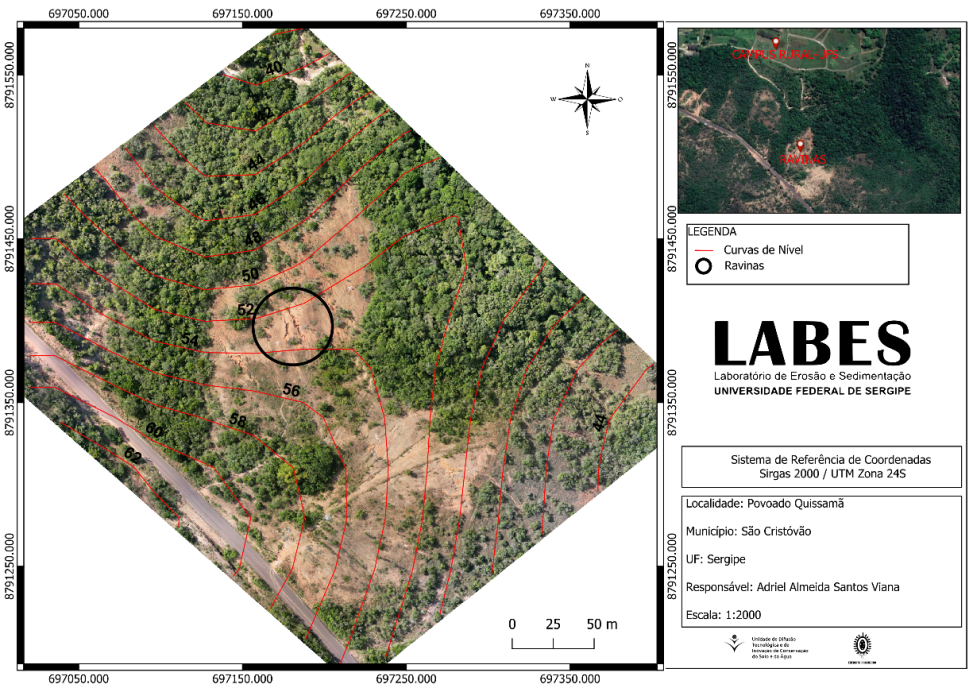
\includegraphics[width=0.9\linewidth,height=\textheight,keepaspectratio]{figuras/fig_00a_area_estudo_aerea.png}

}

\caption{\label{fig-area-aerea}Vista aérea mostrando a paisagem de
pastagem degradada e a ocorrência de feições de erosão linear no
Plintossolo Háplico dos Tabuleiros Costeiros de Sergipe, Nordeste do
Brasil.}

\end{figure}%

Seis feições erosivas ativas (F1 a F6) foram identificadas a partir de
ortomosaicos derivados de VANT com densidade média de nuvem de pontos de
120 pontos/m², e seus parâmetros morfométricos (profundidade, largura e
comprimento) validados por medições diretas em campo com trena (Fig.
Figura~\ref{fig-feicoes-campo}). As profundidades das feições variaram
de 0,40 m (F2) a 1,50 m (F5), correspondendo a profundidades
normalizadas \(H/H_c\) de 0,12 a 0,45 em relação à altura crítica
\(H_c = 3{,}35\) m calculada a partir dos parâmetros geotécnicos medidos
em campo via Equação~\ref{eq-hc}. Esse intervalo indica que o colapso
lateral de talude ainda não se tornou o mecanismo dominante de perda de
solo em nenhuma das feições levantadas, condição que restringe a faixa
de calibração do fator geotécnico \(\gamma\).

\begin{figure}

\centering{

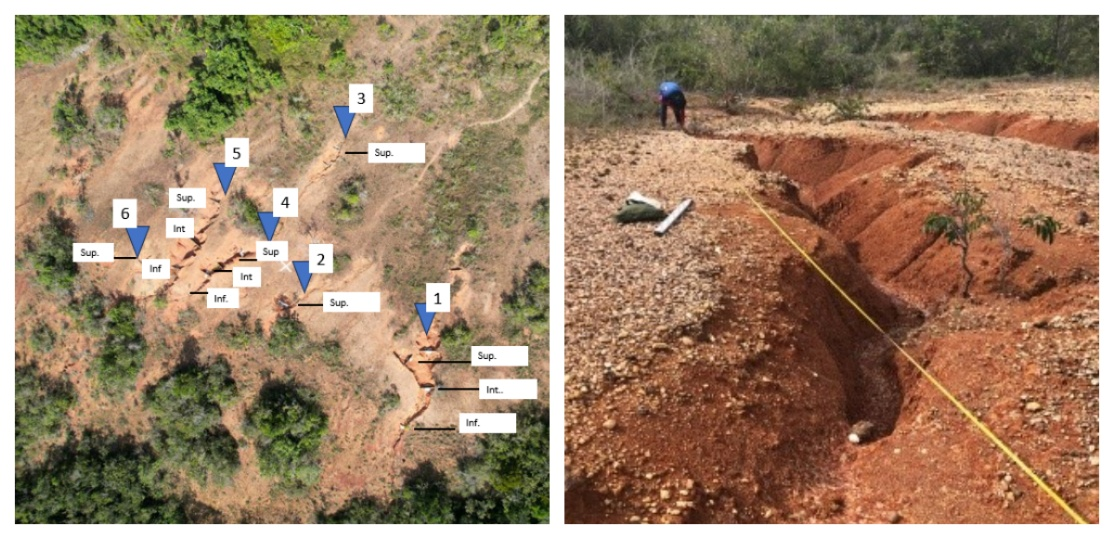
\includegraphics[width=0.9\linewidth,height=\textheight,keepaspectratio]{figuras/fig_00b_feicoes_drone_campo.jpeg}

}

\caption{\label{fig-feicoes-campo}Feições de erosão linear no sítio
experimental.}

\end{figure}%

\emph{Nota: Ortomosaico derivado de VANT mostrando a distribuição
espacial das feições erosivas mapeadas e medição em campo dos parâmetros
morfométricos (profundidade, largura e comprimento) em uma das feições
erosivas ativas.}

Todas as propriedades de entrada do Plintossolo foram obtidas de
medições em campo e análises laboratoriais conduzidas em amostras
coletadas no sítio experimental. A velocidade de infiltração básica
(VIB) foi determinada in situ por ensaios com infiltrômetro de duplo
anel em três horizontes representativos (Ap, BAc e Bf), resultando em
valores de 3,13, 1,53 e 1,59 cm/h, respectivamente, que confirmam que os
horizontes plíntico e subplíntico impõem impedância hidráulica abaixo do
limiar de referência adotado (\(VIB_{ref}\) = 6,0 cm/h). A saturação por
alumínio (\(m_{Al}\)) foi quantificada por análise de fertilidade de
rotina em amostras de cada horizonte genético, com valores variando de
15,2\% no Ap a 99,2\% no Bf, gradiente vertical consistente com a
lixiviação progressiva de bases e concentração de alumínio trocável em
profundidade.

Os parâmetros geotécnicos (coesão efetiva \(c\) = 13,02 kPa, ângulo de
atrito interno \(\phi\) = 34,93° e peso específico saturado
\(\gamma_{sat}\) = 19,93 kN/m³) foram determinados por ensaio de
cisalhamento direto (ASTM D3080) em amostras indeformadas extraídas do
horizonte Bt sob condições saturadas. A erodibilidade \(K_{RUSLE}\) =
0,035 t h MJ\(^{-1}\) mm\(^{-1}\) foi estimada a partir da distribuição
granulométrica, teor de matéria orgânica, código de estrutura e classe
de permeabilidade do horizonte superficial utilizando o nomograma padrão
\citep{wischmeier_et_al_1971}.

Dois perfis virtuais (Latossolo e Argissolo) foram parametrizados a
partir de valores medianos da literatura regional para VIB, saturação
por alumínio, propriedades geotécnicas e \(K_{RUSLE}\)
\citep{silva_et_al_2009, bertoni_lombardi_neto_2017}. O Latossolo opera
como controle negativo
(\(\alpha \approx \beta \approx \gamma \approx 1\)), representando solos
bem drenados sem impedância hidráulica, toxicidade ou feições erosivas
profundas, enquanto o Argissolo funciona como controle parcial,
compartilhando impedância hidráulica moderada no horizonte Bt, porém sem
plintita ou toxicidade extrema por alumínio. As propriedades dos três
perfis são sumarizadas na Tabela 3.

Tabela 3. Propriedades dos três perfis de solo utilizados no
experimento.

\begin{longtable}[]{@{}
  >{\raggedright\arraybackslash}p{(\linewidth - 6\tabcolsep) * \real{0.2500}}
  >{\raggedleft\arraybackslash}p{(\linewidth - 6\tabcolsep) * \real{0.2500}}
  >{\raggedleft\arraybackslash}p{(\linewidth - 6\tabcolsep) * \real{0.2500}}
  >{\raggedleft\arraybackslash}p{(\linewidth - 6\tabcolsep) * \real{0.2500}}@{}}
\toprule\noalign{}
\begin{minipage}[b]{\linewidth}\raggedright
Propriedade
\end{minipage} & \begin{minipage}[b]{\linewidth}\raggedleft
Plintossolo (campo)
\end{minipage} & \begin{minipage}[b]{\linewidth}\raggedleft
Latossolo (virtual)
\end{minipage} & \begin{minipage}[b]{\linewidth}\raggedleft
Argissolo (virtual)
\end{minipage} \\
\midrule\noalign{}
\endhead
\bottomrule\noalign{}
\endlastfoot
VIB superior (cm/h) & 3,13 & 12,0 & 4,5 \\
VIB intermediária (cm/h) & 1,53 & 9,0 & 2,5 \\
VIB inferior (cm/h) & 1,59 & 7,0 & 2,8 \\
\(m_{Al}\) Ap (\%) & 15,2 & 10,0 & 20,0 \\
\(m_{Al}\) subsuperfície (\%) & 84--99 & 20,0 & 45,0 \\
\(c\) (kPa, saturado) & 13,02 & 30,0 & 18,0 \\
\(\phi\) (°) & 34,93 & 30,0 & 32,0 \\
\(\gamma_{sat}\) (kN/m³) & 19,93 & 18,0 & 19,0 \\
\(H_c\) (m) & 3,35 & 5,77 & 4,33 \\
\(H/H_c\) médio & 0,28 & 0,00 & 0,08 \\
\(K_{RUSLE}\) (t h MJ\(^{-1}\) mm\(^{-1}\)) & 0,035 & 0,015 & 0,025 \\
\end{longtable}

\emph{Nota: Os valores do Plintossolo foram obtidos de medições em
campo; os valores do Latossolo e do Argissolo foram parametrizados a
partir da literatura regional.}

\subsection{Delineamento multi-classe}\label{delineamento-multi-classe}

Quanto ao delineamento, o experimento adotará fator fixo principal de
classe de solo, com três níveis, e três parcelas de solo nu por sítio,
dispostas ao longo do gradiente de vertente no sítio-alvo (S1, 3
posições × 1 repetição) e agrupadas em posição única nos sítios-controle
(S2 e S3, 1 posição × 3 repetições). A replicação temporal ao longo de
dois anos hidrológicos (dezenas de eventos erosivos por estação)
compensará o número reduzido de unidades espaciais, gerando centenas de
observações independentes de \(K_{obs}\) por sítio. Os três sítios
experimentais representarão classes pedológicas com gradiente
decrescente de amplificação esperada para os termos \(\alpha\),
\(\beta\) e \(\gamma\).

No arranjo multi-classe, o sítio-alvo (S1) será instalado no Plintossolo
Argilúvico Distrófico descrito na seção 5.1, onde VIB varia de 3,13 cm/h
no terço superior a 1,53 cm/h no intermediário, saturação por alumínio
atinge 99,2\% no horizonte BAc e seis feições erosivas com \(H/H_c\) de
0,12--0,45 foram inventariadas. O sítio-controle negativo (S2) será
instalado em Latossolo Vermelho-Amarelo Distrófico, preferencialmente na
mesma região fisiográfica, selecionado por apresentar VIB tipicamente
superior a 6 cm/h, saturação por alumínio inferior a 30\%, espessura
homogênea do horizonte Bw sem impedância hidráulica abrupta e ausência
de feições erosivas lineares ativas. O sítio-controle parcial (S3) será
instalado em Argissolo Vermelho-Amarelo Distrófico, com gradiente
textural abrupto (horizonte Bt adensado) que reproduz impedância
hidráulica similar à do Plintossolo, porém sem plintita e com saturação
por alumínio intermediária (tipicamente 30--60\%), constituindo classe
que permitirá isolar o efeito do regime hidráulico (\(\alpha\)) das
demais amplificações.

\subsection{Parcelas de erosão e distribuição por
sítio}\label{parcelas-de-erosuxe3o-e-distribuiuxe7uxe3o-por-suxedtio}

As parcelas seguirão o padrão Wischmeier (22,13 m de comprimento na
direção do declive × 1,83 m de largura = 40,5 m²), com calhas coletoras
(Geib) na extremidade inferior conectadas a tanques de armazenamento de
sedimentos. Cada parcela será delimitada por chapas galvanizadas
enterradas a 15 cm para evitar entrada lateral de escoamento. A
superfície das parcelas principais será mantida em pousio (solo nu e
capinado) durante o período experimental para isolar o fator \(K\) dos
efeitos de \(C\) e \(P\) (\(C = P = 1{,}0\)). A configuração da parcela
individual e a distribuição das 14 unidades nos três sítios são
apresentadas na Fig. Figura~\ref{fig-esquema}.

\begin{figure}[H]

\centering{

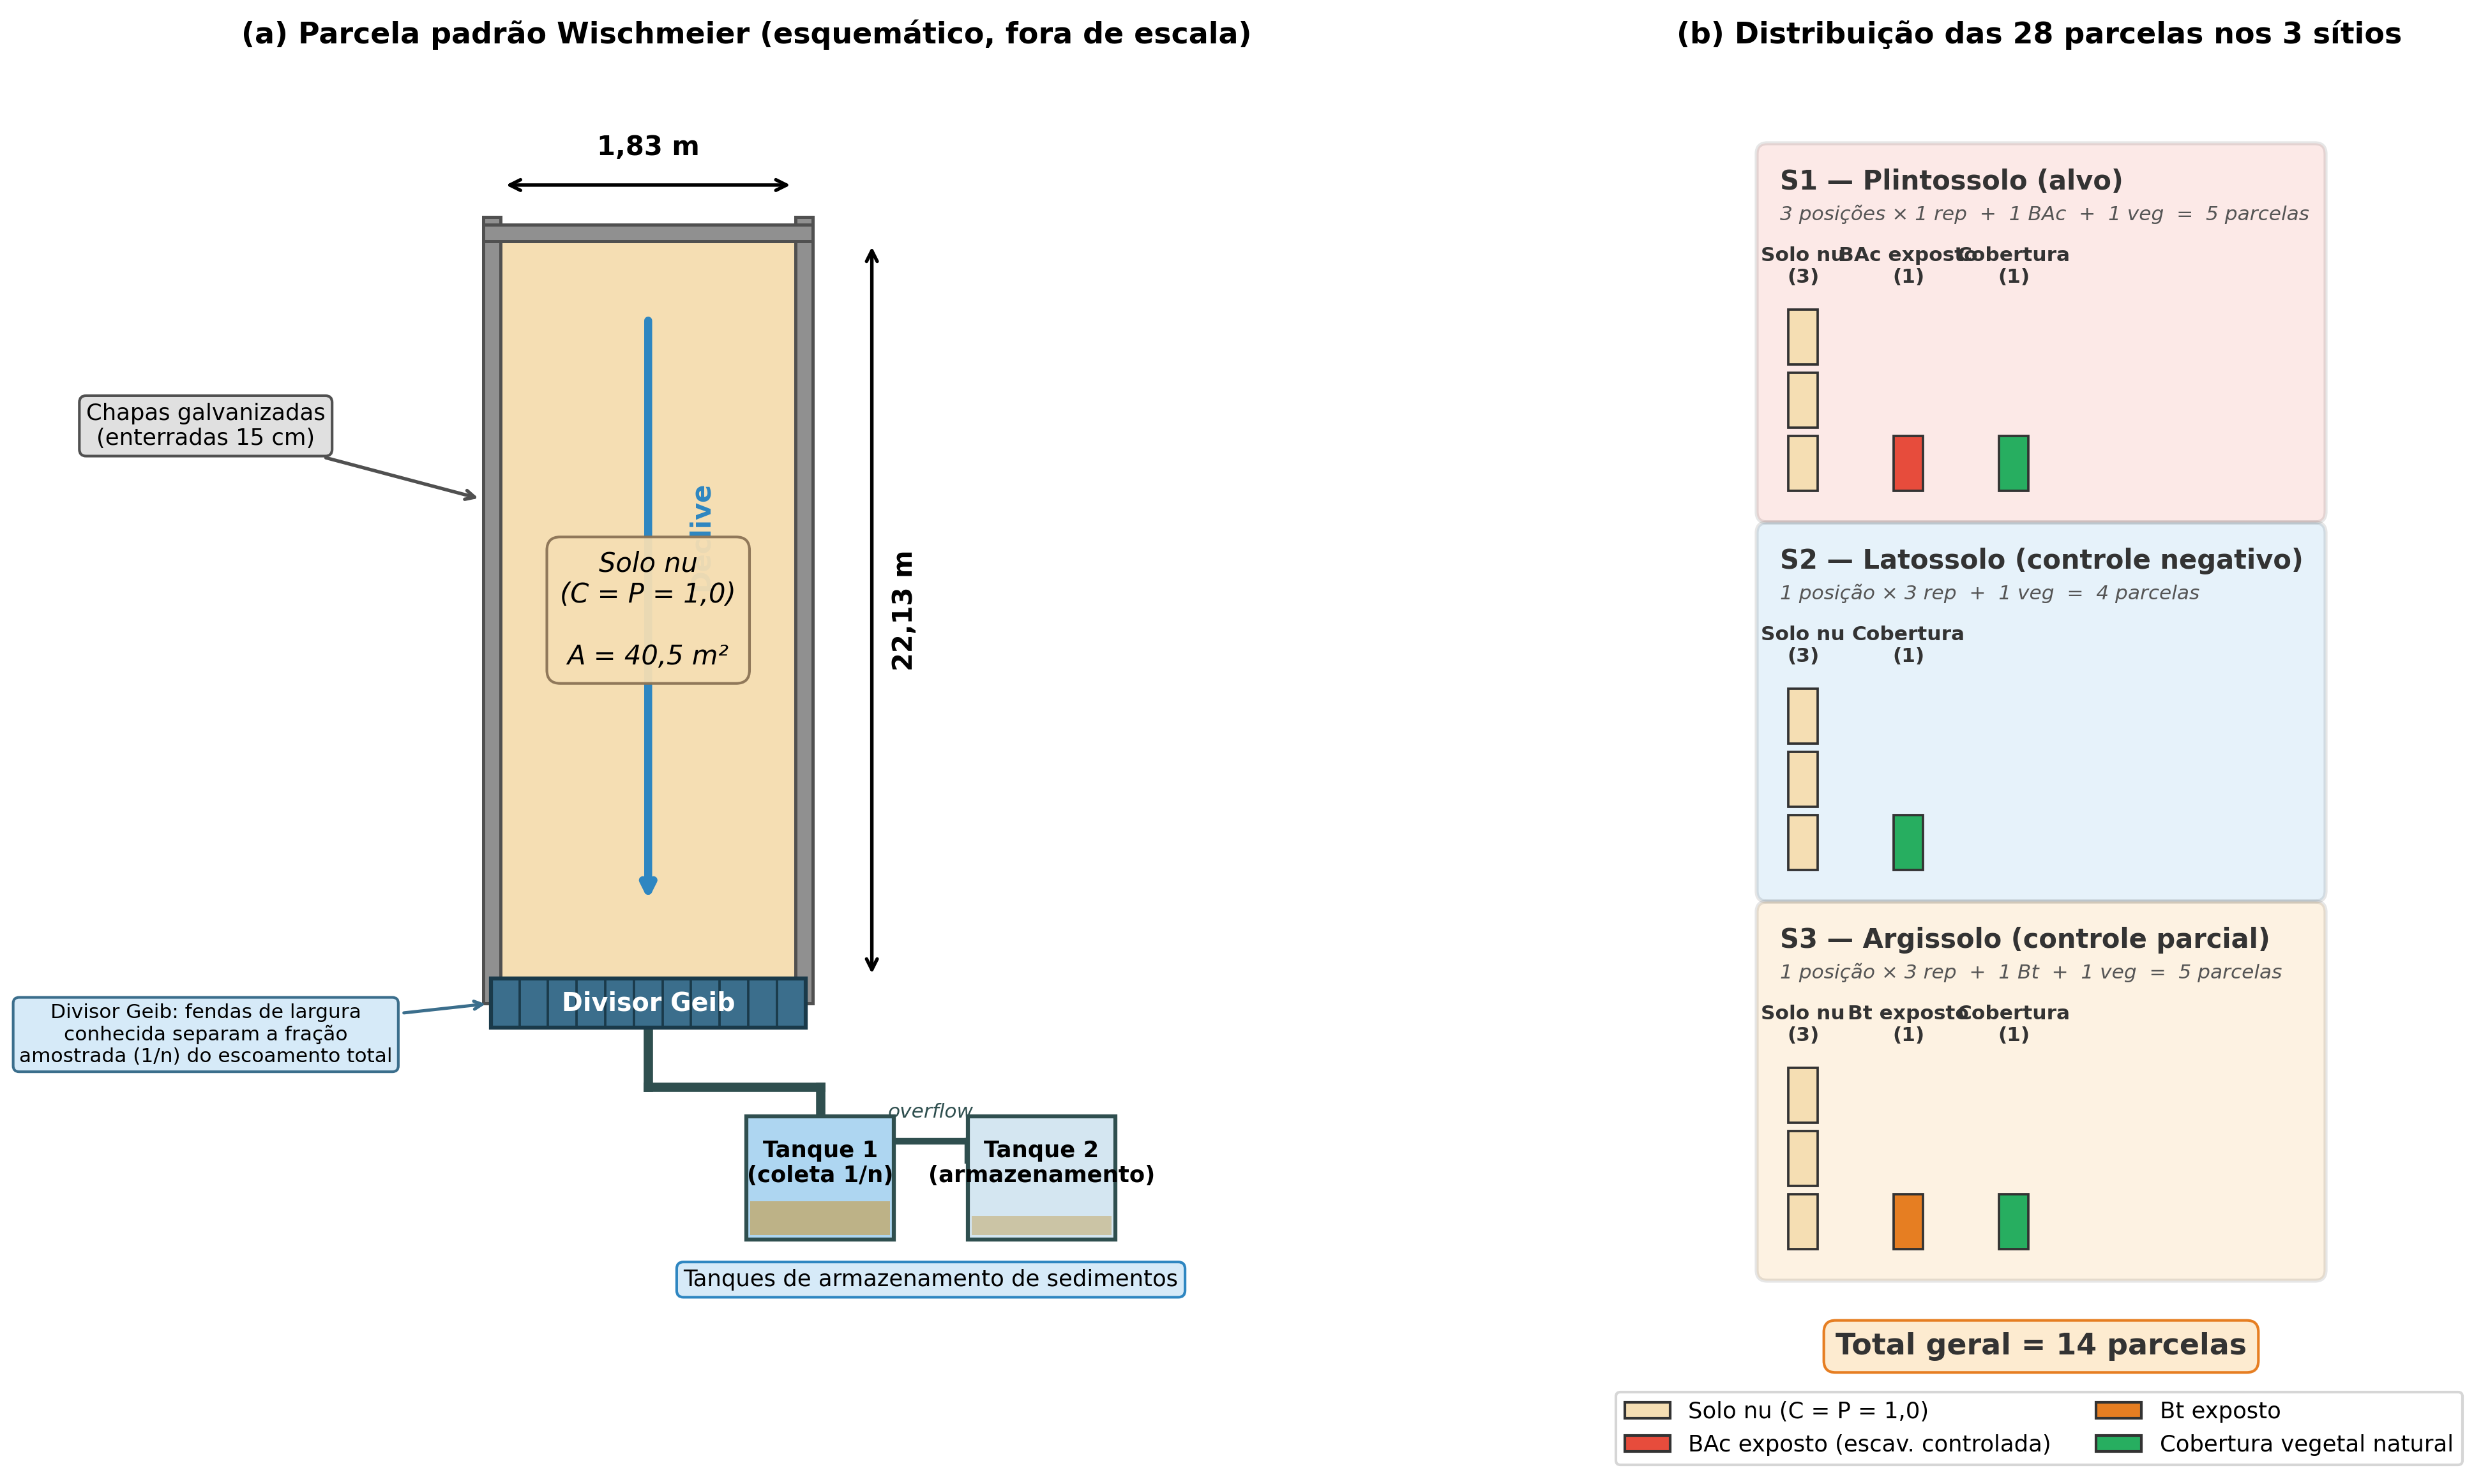
\includegraphics[width=1\linewidth,height=\textheight,keepaspectratio]{figuras/fig_esquema_parcela_experimento.png}

}

\caption{\label{fig-esquema}Esquema do experimento de erosão. (a)
Parcela padrão Wischmeier com divisor Geib, tanques de coleta e
armazenamento de sedimentos e chapas galvanizadas de delimitação
lateral. (b) Distribuição das parcelas nos três sítios pedológicos.}

\end{figure}%

Espacialmente, a distribuição apresentada na Fig.
Figura~\ref{fig-esquema} organiza o contraste entre o sítio-alvo em
Plintossolo e os dois sítios-controle, preservando comparabilidade
geomorfológica suficiente para estimar separadamente as contribuições de
\(\alpha\), \(\beta\) e \(\gamma\).

Operacionalmente, o sistema de coleta com divisor Geib adotado em cada
parcela é detalhado na Fig. Figura~\ref{fig-geib}, em que o
fracionamento do deflúvio excedente entre tanques amplia a capacidade de
armazenamento sem perda de representatividade amostral
\citep{melo_neto_et_al_2021}.

\begin{figure}[H]

\begin{minipage}{0.50\linewidth}

\centering{

\pandocbounded{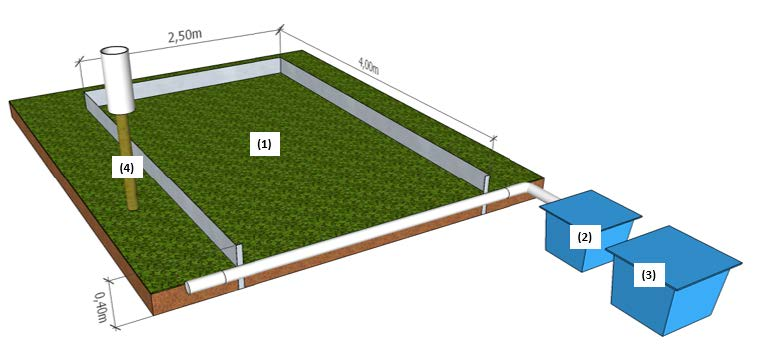
\includegraphics[keepaspectratio]{figuras/geib_a.jpeg}}

}

\subcaption{\label{fig-geib-a}Croqui da parcela com divisor Geib e
tanques de coleta}

\end{minipage}%
%
\begin{minipage}{0.50\linewidth}

\centering{

\pandocbounded{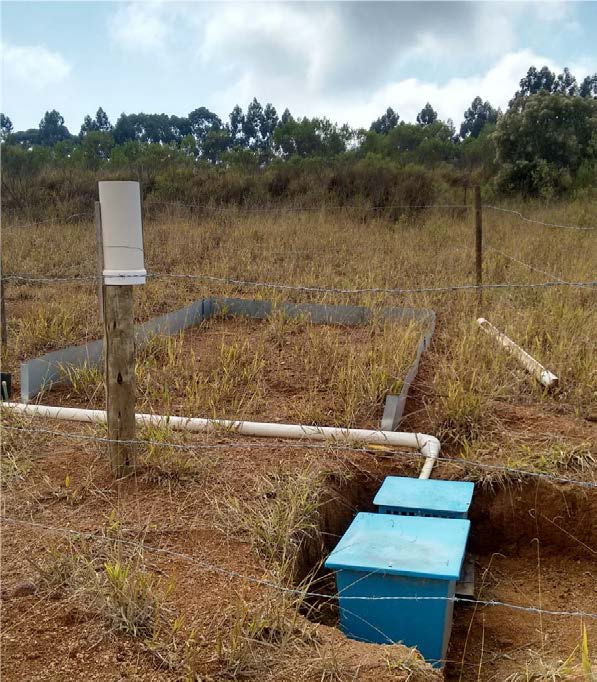
\includegraphics[keepaspectratio]{figuras/geib_b.jpeg}}

}

\subcaption{\label{fig-geib-b}Parcela instalada em campo}

\end{minipage}%

\caption{\label{fig-geib}Parcela de monitoramento de erosão hídrica do
solo com divisor Geib. (a) Croqui esquemático e (b) vista de campo.
Adaptado de \citet{melo_neto_et_al_2021}.}

\end{figure}%

No sítio S1 (Plintossolo), o arranjo compreenderá 3 parcelas em solo nu
(3 posições × 1 repetição, ao longo do gradiente de VIB), 1 parcela com
horizonte BAc exposto por escavação controlada para isolar o efeito de
\(\beta\) e 1 parcela com cobertura vegetal natural para quantificar a
interação \(\beta \times C\), totalizando 5 parcelas. No sítio S2
(Latossolo), 3 parcelas em solo nu (1 posição × 3 repetições) e 1
parcela com cobertura vegetal constituirão o arranjo mínimo necessário
para estimar \(K_{obs}\) e verificar se \(\delta \approx 1{,}0\) (4
parcelas). No sítio S3 (Argissolo), 3 parcelas em solo nu (1 posição × 3
repetições), 1 parcela com horizonte Bt exposto e 1 parcela com
cobertura vegetal permitirão isolar a contribuição do gradiente textural
(5 parcelas). O total geral do experimento será de 14 parcelas.

\subsection{Protocolo de ensaios}\label{protocolo-de-ensaios}

\subsubsection{Ensaios comuns às três
classes}\label{ensaios-comuns-uxe0s-truxeas-classes}

Em campo, o protocolo de monitoramento compreenderá quatro componentes
simultâneos realizados durante dois anos hidrológicos consecutivos
(abril a março), cobrindo a totalidade da estação chuvosa
(abril--agosto) e o período seco (setembro--março). A medição contínua
de precipitação utilizará pluviógrafo de báscula (resolução 0,2 mm,
intervalo de registro de 5 min) instalado na crista de cada vertente,
para cálculo do índice de erosividade \(R\) (EI\(_{30}\)) por evento
\citep{wischmeier_smith_1978}. A coleta de sedimentos em tanques de
armazenamento ocorrerá após cada evento erosivo com precipitação
superior a 10 mm, quantificando a perda de solo por parcela em t
ha\(^{-1}\) evento\(^{-1}\). A VIB será medida sazonalmente por
infiltrômetro de anéis duplos (3 posições × 3 repetições por sítio) e
amostras de solo serão coletadas para determinação de granulometria
completa (com areia muito fina separada), matéria orgânica
(Walkley-Black ou combustão seca), complexo sortivo completo (pH, Al³⁺,
H+Al, CTC, V\%, saturação por alumínio \(m\)), limites de Atterberg (LL,
LP, IP), densidade do solo e de partículas (\(\gamma_{sat}\)) e
mineralogia por difração de raios X (DRX) do horizonte diagnóstico. Cada
sítio contará com levantamento topográfico por estação total ou GNSS-RTK
para determinação dos fatores \(L\) e \(S\).

Sob condição saturada, o ensaio de cisalhamento direto (tensões normais
de 25, 50, 100 e 200 kPa) será realizado em amostras indeformadas do
horizonte diagnóstico de cada classe (Fig. Figura~\ref{fig-sitio}),
fornecendo coesão (\(c\)) e ângulo de atrito (\(\phi\)) para cálculo de
\(H_c\) pela Equação~\ref{eq-hc}. A condutividade hidráulica saturada
por horizonte (permeâmetro de carga constante) será determinada em
amostras indeformadas de dois a três horizontes por perfil, validando a
presença ou ausência de impedância hidráulica abrupta.

\begin{figure}

\centering{

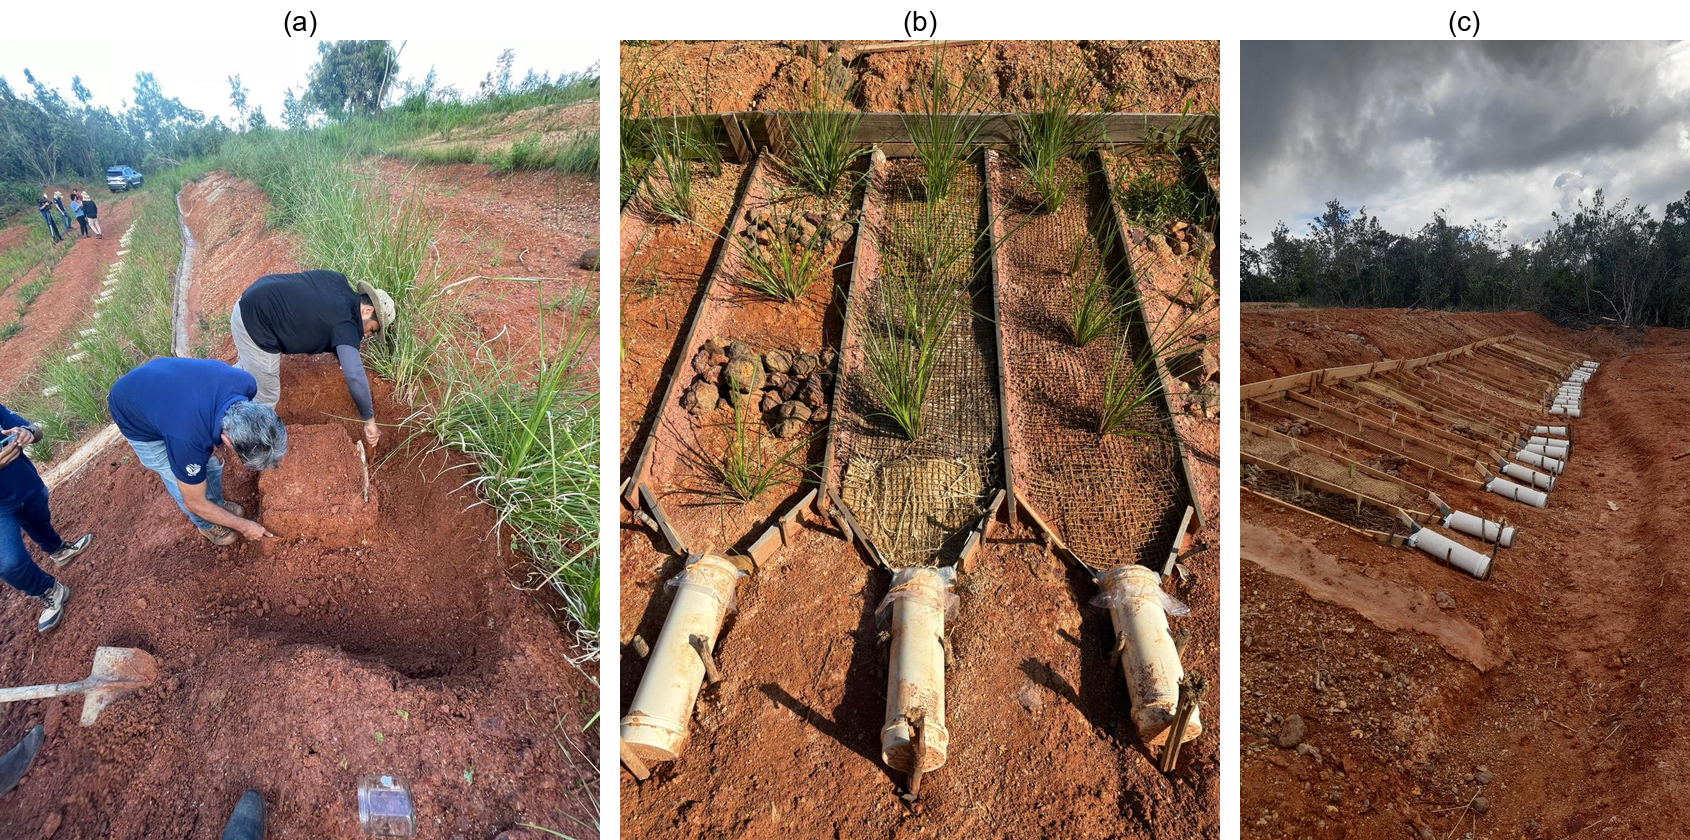
\includegraphics[width=1\linewidth,height=\textheight,keepaspectratio]{figuras/fig_09_sitio_experimental.png}

}

\caption{\label{fig-sitio}Elementos do sítio experimental em Plintossolo
Háplico, Tabuleiros Costeiros de Sergipe. (a) Bloco indeformado extraído
para ensaio de cisalhamento direto (\(c\) = 13,02 kPa, \(\phi\) =
34,93°). (b) Parcelas de coleta de sedimentos posicionadas na base do
talude erosivo. (c) Vista geral do talude com feições erosivas ativas.}

\end{figure}%

Complementarmente às parcelas Wischmeier, microparcelas instrumentadas
(1 m² de área coletora) serão instaladas em três posições da vertente de
cada sítio, equipadas com pluviógrafo de disdrômetro a laser (resolução
temporal de 1 min, energia cinética por classe de diâmetro de gota) para
capturar a distribuição intra-evento da intensidade e da energia
cinética da chuva. A conectividade hidrossedimentológica em Plintossolos
depende fortemente de pulsos intensos cuja duração raramente excede 15
min, de modo que a resolução padrão de 5 min pode subestimar picos de
intensidade que disparam escoamento hortoniano e destacamento por
impacto de gotas no horizonte BAc \citep{kinnell_2005}. As microparcelas
fornecerão observações de alta frequência que alimentarão diretamente o
modelo de mistura da Equação~\ref{eq-fd}, pois a energia cinética
acumulada por evento constitui a variável de entrada para estimativa da
energia de desagregação específica (\(E_d\)) e calibração dos
coeficientes \(a_1\)--\(a_4\).

Sessões de chuva simulada em laboratório complementarão o monitoramento
de campo, replicando os quantis superiores da distribuição de
intensidade observada (intensidades correspondentes aos percentis 90, 95
e 99 da série pluviográfica do sítio) sobre amostras indeformadas de
cada horizonte diagnóstico, em condição natural e após tratamento com
ditionito-citrato-bicarbonato para remoção seletiva de ferro livre. O
simulador de chuva operará com bicos oscilantes a 3 m de altura,
produzindo gotas com distribuição de tamanho e energia cinética
comparáveis à chuva natural tropical (intensidades de 30, 60, 90 e 120
mm/h, duração de 30 min por intensidade). A comparação entre amostras
naturais e desferrificadas permitirá estimar a fração dispersável
(\(f_d\)) e a energia de desagregação (\(E_d\)) para cada classe de
solo, calibrando os parâmetros do modelo de mistura sob condições
controladas antes de aplicá-los aos dados de campo (Fig.
Figura~\ref{fig-chuva-simulada}).

\begin{figure}

\centering{

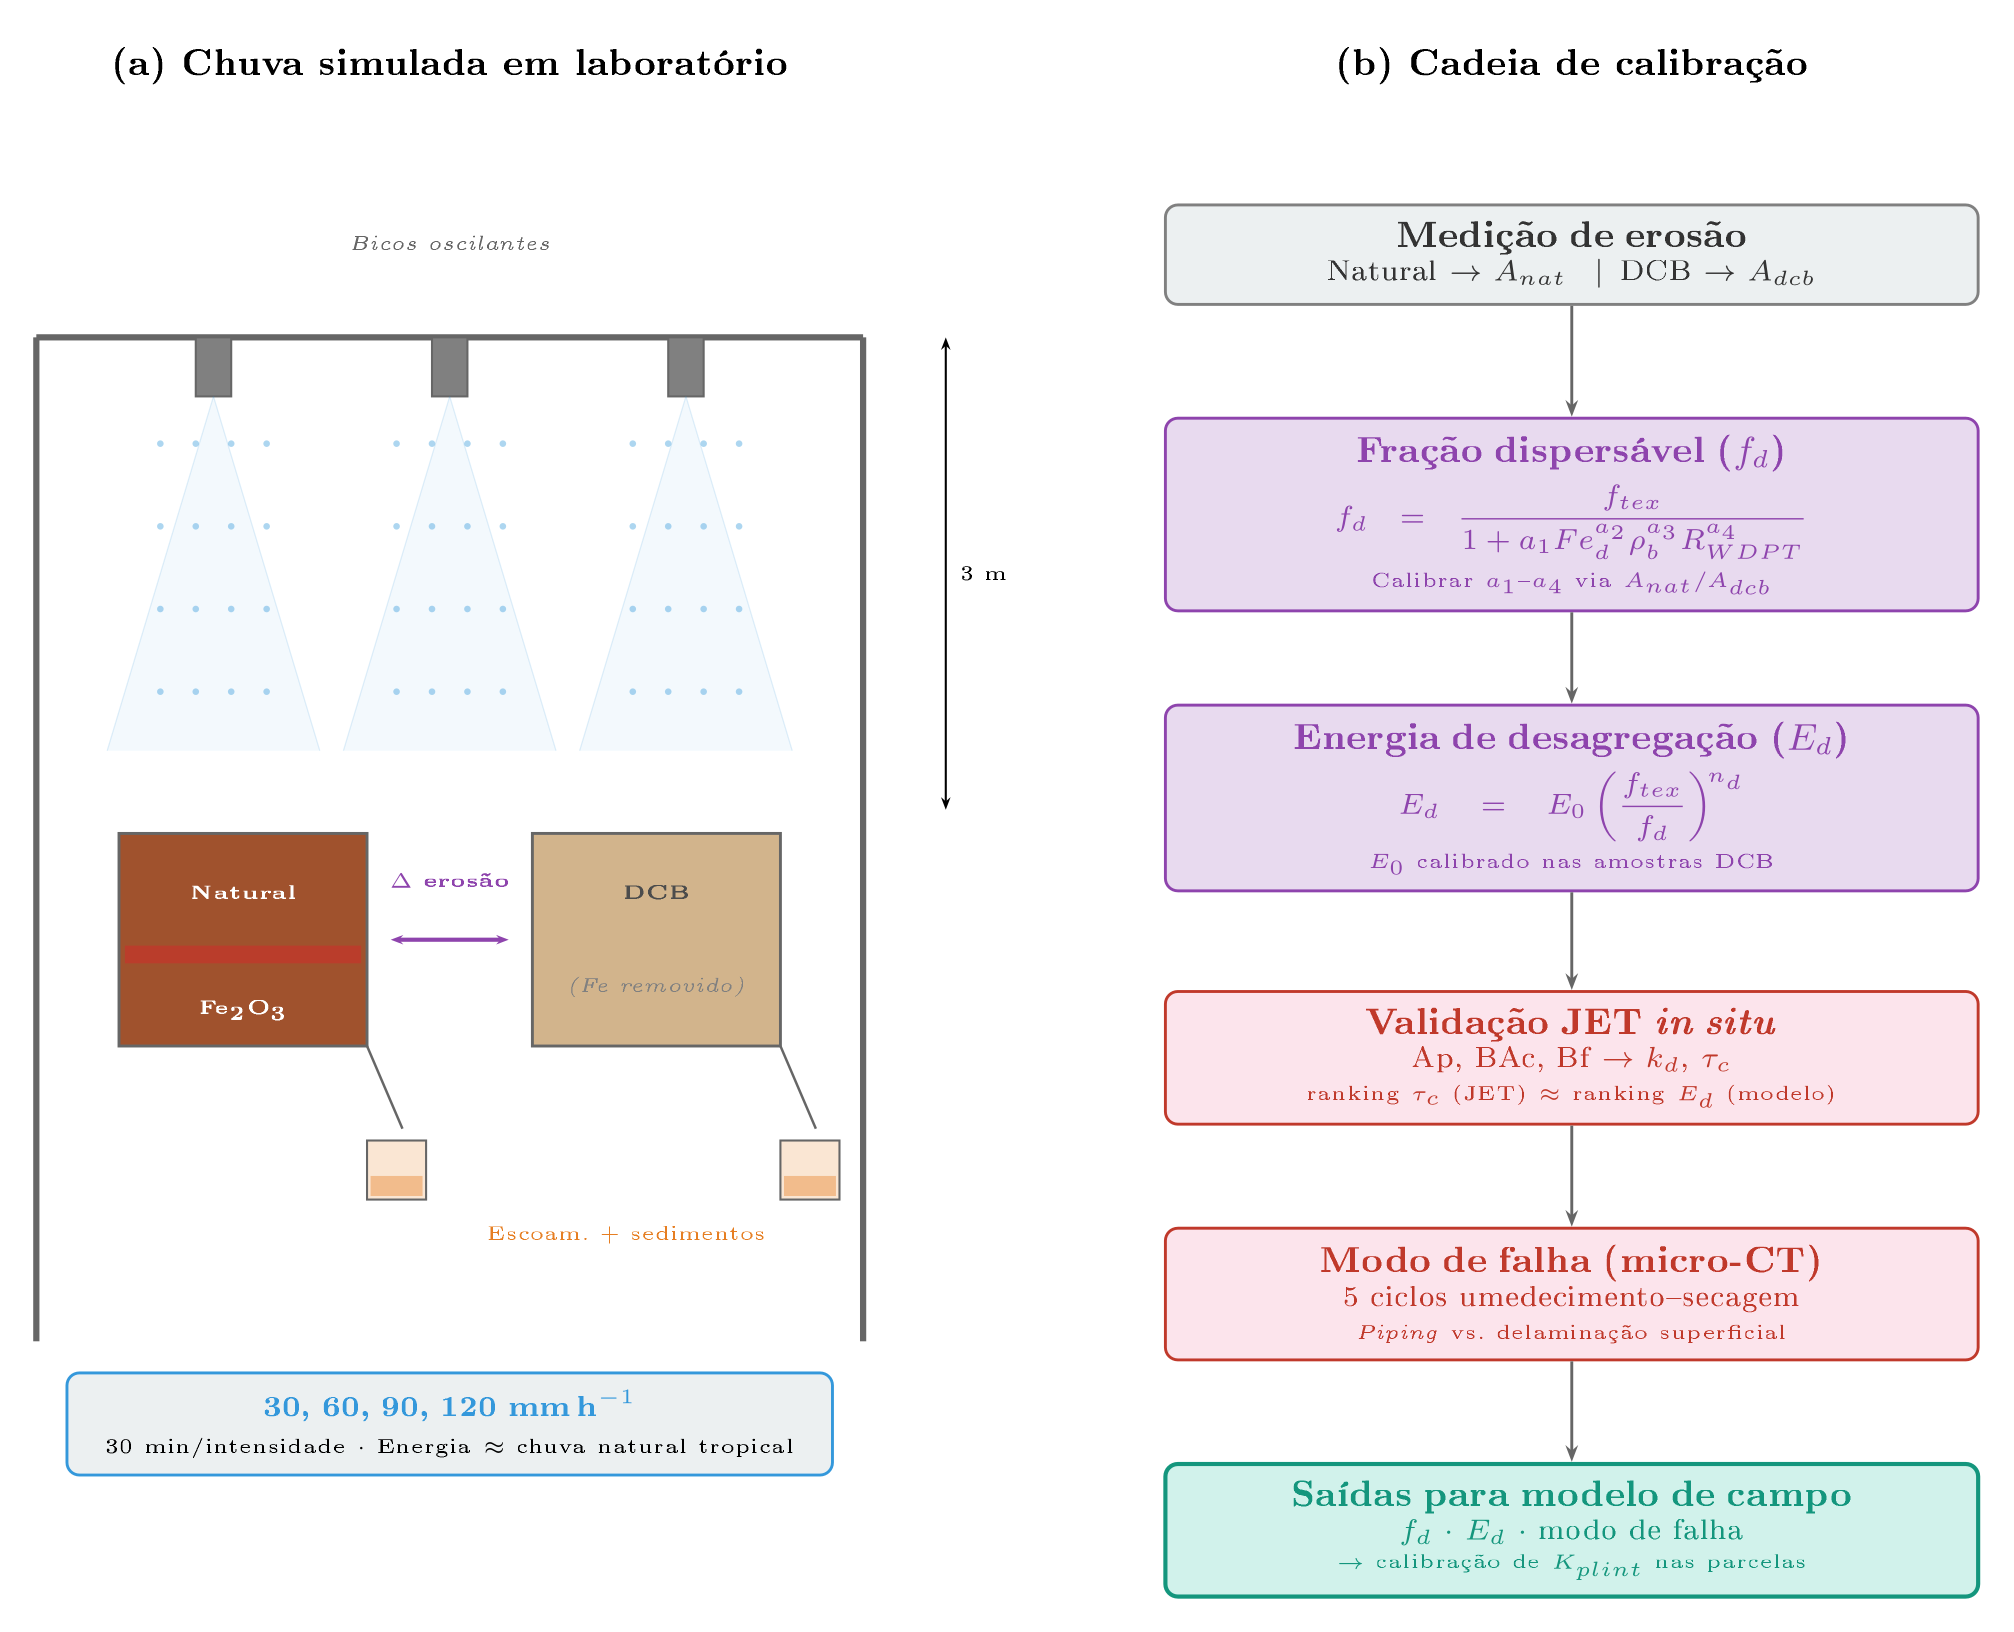
\includegraphics[width=1\linewidth,height=\textheight,keepaspectratio]{figuras/fig_esquema_chuva_simulada.png}

}

\caption{\label{fig-chuva-simulada}Configuração do ensaio de chuva
simulada e cadeia de calibração. (a) Estrutura laboratorial com bicos
oscilantes a 3 m de altura, amostras naturais e tratadas com DCB, e
coleta de escoamento e sedimentos sob quatro intensidades (30--120 mm
h\(^{-1}\)). (b) Cadeia de calibração desde a medição de erosão até a
saída para o modelo de campo, passando pela fração dispersável
(\(f_d\)), energia de desagregação (\(E_d\)), validação JET e modo de
falha por microtomografia.}

\end{figure}%

\subsubsection{Ensaios específicos por
classe}\label{ensaios-especuxedficos-por-classe}

No sítio S1 (Plintossolo), o monitoramento de profundidade das feições
adjacentes às parcelas utilizará pinos de erosão (20 pinos por feição,
espaçamento de 1 m longitudinal × 0,5 m transversal, leituras
quinzenais), para quantificar o incremento volumétrico atribuível a
colapso de taludes e incisão vertical. A parcela com horizonte BAc
exposto por escavação controlada permitirá isolar o efeito da toxicidade
extrema (\(m\) = 99,2\%) sobre a erodibilidade observada. Um inventário
completo das feições erosivas (profundidade, largura, comprimento,
\(H/H_c\)) será realizado semestralmente.

Para elucidar o modo de falha do material cimentado, ensaios de Jet
Erosion Test (JET) invertido serão realizados in situ nos taludes das
feições F1, F4 e F5, que apresentam os maiores valores de \(H/H_c\), com
jatos aplicados em três horizontes distintos (Ap, BAc e Bf) para
determinação do coeficiente de erodibilidade do solo ao jato (\(k_d\),
cm³ N\(^{-1}\) s\(^{-1}\)) e da tensão cisalhante crítica (\(\tau_c\),
Pa) em cada camada \citep{hanson_cook_2004}. A combinação dos parâmetros
JET com a fração dispersável (\(f_d\)) estimada pelo modelo de mistura
da Equação~\ref{eq-fd} permitirá verificar se a resistência ao
cisalhamento do material cimentado é consistente com a predição do
modelo mecanístico, fechando a cadeia causal entre mineralogía dos
óxidos, cimentação e erodibilidade efetiva.

Complementarmente, amostras indeformadas extraídas com caixa metálica
(15 × 15 × 30 cm) dos mesmos horizontes serão submetidas a tomografia
computadorizada de raios X (micro-CT, resolução de 50 µm) antes e após
ciclos controlados de umedecimento e secagem (5 ciclos, saturação por
capilaridade seguida de secagem a 40 °C por 48 h). A tomografia
fornecerá perfil vertical tridimensional da progressão da ruptura,
permitindo distinguir se o colapso da matriz cimentada se dá
predominantemente por piping (desenvolvimento de canais internos ao
longo de macroporos obstruídos por óxidos) ou por delaminação
superficial (destacamento laminar progressivo da crosta ferruginosa),
informação relevante para a escolha de práticas de manejo e para a
interpretação física do expoente \(n_d\) do modelo de energia de
desagregação (Equação~\ref{eq-ed}). A fração de porosidade conectada e o
diâmetro médio de poros antes e após os ciclos constituirão variáveis
auxiliares para validação do modelo de mistura em condições de campo.

Em escala de vertente, o rastreamento da evolução das feições erosivas
utilizará fotogrametria dronada bimestral (VANT multirrotor com câmera
RGB de 20 MP, altura de voo de 30 m, GSD de 1,2 cm, 8 pontos de controle
georreferenciados por GNSS-RTK), produzindo modelos digitais de
superfície (MDS) e ortomosaicos de alta resolução a cada campanha. A
diferenciação temporal entre MDS consecutivos (DoD, DEM of Difference,
com limiar de detecção de mudança de ±3 cm) quantificará o alongamento
linear, o recuo de cabeceira e a variação volumétrica de cada feição ao
longo do período experimental, permitindo correlacionar a taxa de
progressão das feições com a integral temporal da energia de escoamento
concentrado acumulada entre campanhas, vinculando diretamente o fator
\(K_{plint}\) recalibrado ao desempenho hidrossedimentológico observado
em escala de vertente.

No sítio S2 (Latossolo), não se preveem pinos de erosão nem parcelas com
horizonte exposto, dado que a hipótese H5 prediz
\(\delta \approx 1{,}0\) (ausência de amplificação). A mineralogia por
DRX confirmará a presença de gibbsita e oxi-hidróxidos de ferro
responsáveis pela microagregação estável típica de Latossolos
\citep{silva_et_al_2009}.

No sítio S3 (Argissolo), pinos de erosão serão instalados apenas se
feições erosivas lineares forem identificadas durante o inventário
inicial. Uma parcela com horizonte Bt exposto permitirá avaliar se a
impedância hidráulica do gradiente textural abrupto, sem toxicidade
extrema por alumínio, é suficiente para gerar \(\alpha > 1\)
isoladamente.

\subsection{\texorpdfstring{Cálculo de
\(K_{obs}\)}{Cálculo de K\_\{obs\}}}\label{cuxe1lculo-de-k_obs}

Para cada parcela em solo nu (\(C = P = 1\)), \(K_{obs}\) será obtido
por inversão da Equação~\ref{eq-usle} (Equação~\ref{eq-kobs}).

\begin{equation}\phantomsection\label{eq-kobs}{
K_{obs} = \dfrac{A_{obs}}{R \times L \times S}
}\end{equation}

onde \(A_{obs}\) é a perda de solo medida (t ha\(^{-1}\) ano\(^{-1}\)),
\(R\) a erosividade acumulada anual calculada a partir dos registros
pluviográficos, \(L\) o fator de comprimento calculado pela fórmula de
\citet{renard_et_al_1997} e \(S\) o fator de declividade medido por
estação total em cada parcela.

Para o mesmo material, o fator \(K_{RUSLE}\) será estimado pela
Equação~\ref{eq-nomograma} a partir dos dados de granulometria, matéria
orgânica e classificação de estrutura e permeabilidade do horizonte
exposto. A razão \(\delta = K_{obs}/K_{RUSLE}\) quantificará a
discrepância entre erodibilidade observada e prevista, que constitui a
variável-resposta do modelo de correção.

\subsection{Procedimento de
calibração}\label{procedimento-de-calibrauxe7uxe3o}

Os cinco parâmetros livres (\(n_1\), \(\beta_{max}\), \(k_2\), \(k_3\),
\(n_3\)) serão calibrados por protocolo sequencial em cinco etapas,
explorando a estrutura multi-classe para isolar cada termo.

Sinteticamente, a Fig. Figura~\ref{fig-fluxograma} reúne a sequência
operacional da calibração e a articulação entre o modelo multiplicativo
e o submodelo laboratorial auxiliar.

\begin{figure}[H]

\centering{

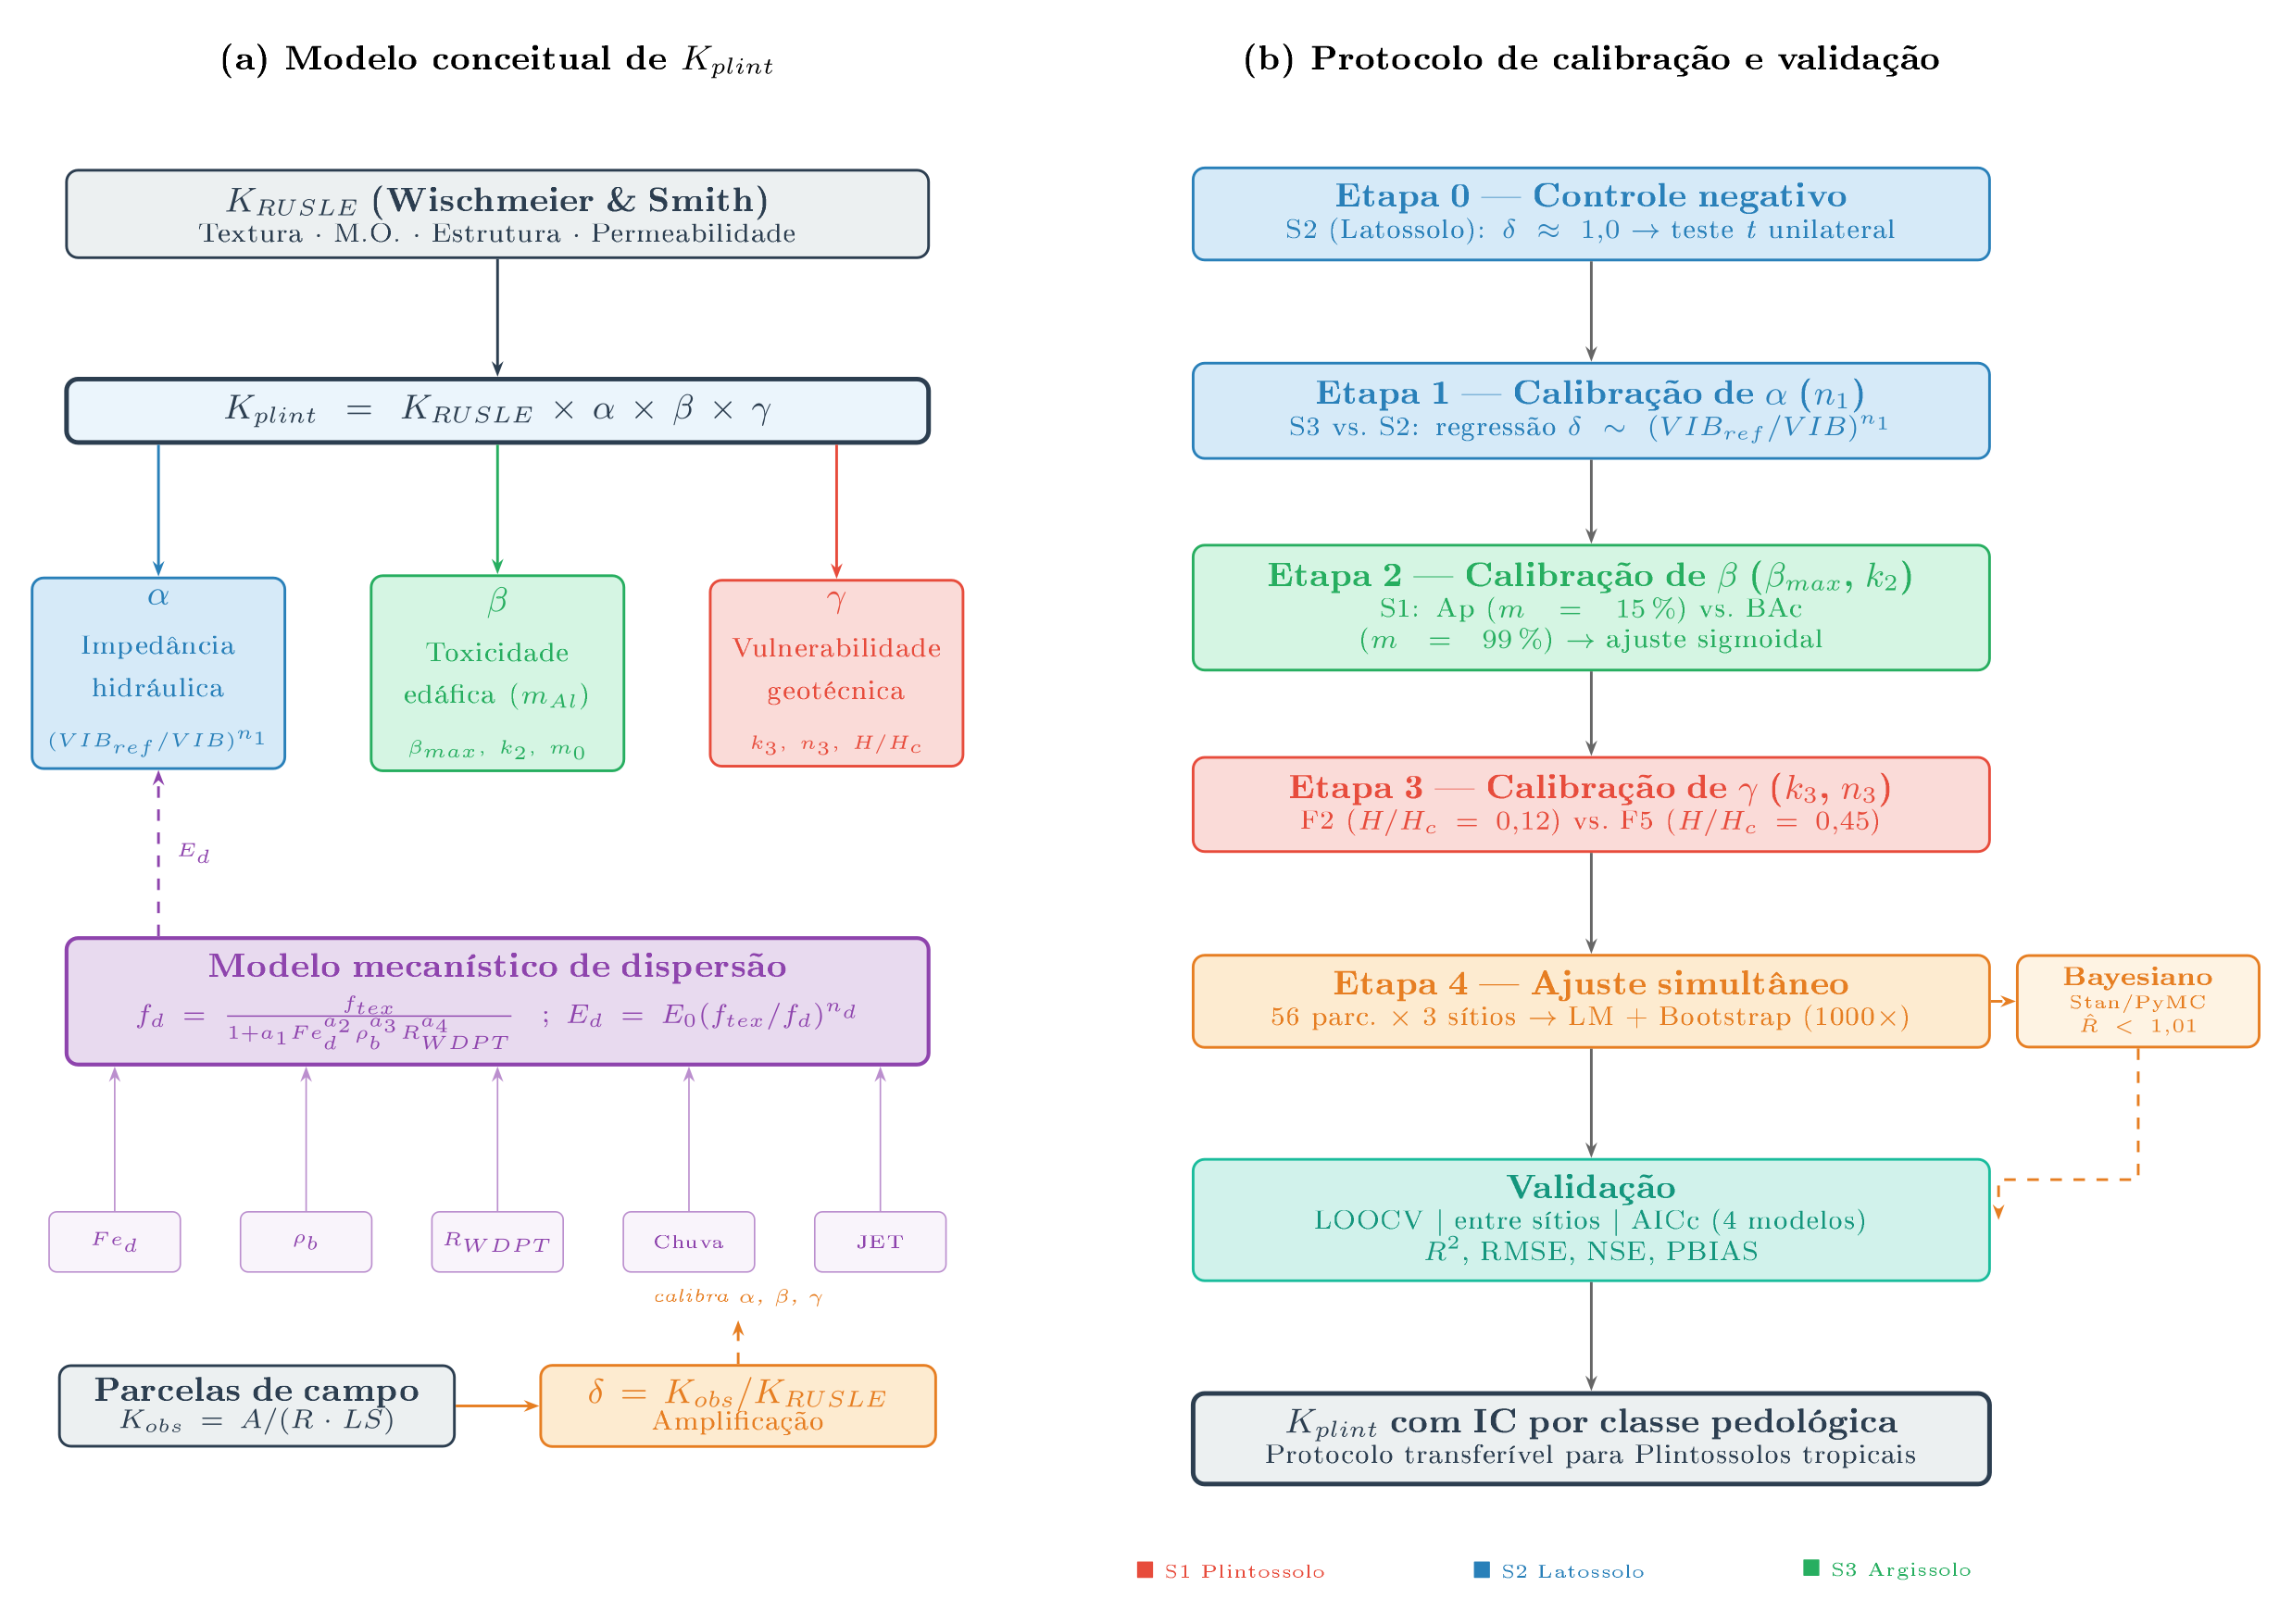
\includegraphics[width=0.8\linewidth,height=\textheight,keepaspectratio]{figuras/fig_fluxograma_kplint.png}

}

\caption{\label{fig-fluxograma}Estrutura conceitual e protocolo de
calibração do modelo \(K_{plint}\). (a) Arquitetura multiplicativa do
fator de correção com os três mecanismos amplificadores (\(\alpha\),
\(\beta\), \(\gamma\)), modelo mecanístico de dispersão e variáveis de
entrada. (b) Protocolo de calibração sequencial em cinco etapas, com
braço bayesiano hierárquico e validação cruzada entre sítios.}

\end{figure}%

No controle negativo, \(\delta_{S2}\) (Latossolo) será comparado com a
unidade para verificar se o nomograma representa adequadamente a
erodibilidade observada nessa classe. Se \(\delta_{S2}\) permanecer
próximo de 1\{,\}0, a discrepância observada nos demais sítios será
interpretada como resposta das propriedades específicas de cada solo. Se
houver desvio sistemático em relação à unidade, os parâmetros ajustados
nos sítios S1 e S3 serão interpretados em relação ao comportamento de
referência do Latossolo, e não como correções absolutas.

Entre Argissolo e Latossolo, \(\delta_{S3}\) (com \(\alpha > 1\), mas
\(\beta \approx 1\) e \(\gamma \approx 1\)) será comparado com
\(\delta_{S2}\) (com \(\alpha \approx 1\)). A razão
\(\delta_{S3}/\delta_{S2}\), atribuível predominantemente a \(\alpha\),
fornecerá a base empírica para quantificar a amplificação associada ao
rebaixamento de \(VIB\) nas parcelas em solo nu do Argissolo.

Entre os horizontes Ap e BAc do Plintossolo, as parcelas do sítio S1 com
Ap (\(m\) = 15,2\%) e BAc exposto (\(m\) = 99,2\%), na mesma posição da
vertente e sob VIB controlada, fornecerão a base para calibração de
\(\beta\). A diferença de \(\delta\) entre horizontes, descontado o
efeito de \(\alpha\) já isolado, será atribuída à toxicidade edáfica,
enquanto a comparação entre parcelas com Bt exposto no Argissolo (S3,
\(m\) intermediário) e parcelas com BAc exposto no Plintossolo (S1,
\(m\) extremo) servirá como verificação independente da direção e da
magnitude dessa penalização.

Nas parcelas do sítio S1 adjacentes às feições F2 e F5, com \(H/H_c\)
contrastante (0,12 vs.~0,45), a perda total de solo (parcela + pinos de
erosão) fornecerá a base para isolar a contribuição de \(\gamma\). Como
\(\alpha\) e \(\beta\) já terão sido estimados nas etapas anteriores, o
resíduo \(\delta_{residual} = \delta_{obs} / (\alpha \times \beta)\)
será interpretado como expressão da vulnerabilidade geotécnica associada
à aproximação do limiar de ruptura.

Por fim, a integração das cinco etapas utilizará todos os valores de
\(\delta_{obs}\) disponíveis nos três sítios (n = 56 parcelas), partindo
das estimativas obtidas nos contrastes marginais para produzir um
conjunto único de parâmetros capaz de representar simultaneamente os
mecanismos hidráulico, edáfico e geotécnico.

Critérios de ajuste, testes de hipótese, comparação entre modelos e
métricas de desempenho empregados em cada etapa são apresentados de
forma concentrada na seção Análises estatísticas.

\subsection{Análises estatísticas}\label{anuxe1lises-estatuxedsticas}

Como variável-resposta de todas as análises, será adotada a razão
\(\delta = K_{obs}/K_{RUSLE}\), interpretada como amplificação da
erodibilidade observada em relação ao valor previsto pelo nomograma. No
controle negativo, \(\delta_{S2}\) será comparado com a unidade por
teste t unilateral (\(\alpha\) = 0,05), verificando se o Latossolo se
mantém dentro do domínio de adequação da USLE/RUSLE. A estimação
marginal de \(\alpha\) será conduzida por regressão não linear
univariada de \(\delta_{S3}/\delta_{S2}\) contra
\(VIB_{ref}/VIB_{local}\), enquanto \(\beta\) será ajustado pela forma
sigmoidal da Equação~\ref{eq-beta} usando o contraste entre Ap e BAc no
Plintossolo e, de modo complementar, o contraste entre Bt exposto no
Argissolo e BAc exposto no Plintossolo. A contribuição de \(\gamma\)
será estimada por regressão não linear de
\(\delta_{residual} = \delta_{obs}/(\alpha \times \beta)\) contra
\(H/H_c\) nas feições F2 e F5.

Na etapa de integração, a formulação completa da
Equação~\ref{eq-kplint-exp} será ajustada simultaneamente por mínimos
quadrados não lineares via algoritmo de Levenberg-Marquardt, utilizando
os 56 valores de \(\delta_{obs}\) disponíveis nos três sítios e tomando
como valores iniciais as estimativas obtidas nas etapas marginais. A
incerteza paramétrica será quantificada por bootstrap paramétrico com
1000 reamostras. Complementarmente, será ajustado um modelo hierárquico
bayesiano em que cada microparcela receberá parâmetros parcialmente
compartilhados (\(n_1\), \(\beta_{max}\), \(k_2\), \(k_3\), \(n_3\)) por
prioris centradas na média da classe pedológica, separando variação
intra-sítio e inter-sítio. A intensidade de pico da chuva
(\(I_{max,15}\), mm h\(^{-1}\)) e a energia cinética acumulada por
evento (\(E_k\), MJ ha\(^{-1}\)) entrarão como preditores hierárquicos
de segundo nível, condicionando a distribuição a posteriori de \(n_1\) e
\(n_d\) e reduzindo extrapolação para regimes pluviométricos não
observados. A implementação utilizará Stan ou PyMC com quatro cadeias de
5000 iterações, descartando as primeiras 1000 como aquecimento, e
adotará \(\hat{R}\) \textless{} 1,01 e tamanho efetivo de amostra
\textgreater{} 400 como critérios de convergência
\citep{gelman_et_al_2013}.

Em termos preditivos, a validação combinará procedimento leave-one-out
sobre o conjunto total de observações e validação cruzada entre sítios,
calibrando o modelo com dados de dois sítios e testando no terceiro. O
desempenho será quantificado por \(R^2\), RMSE, NSE e PBIAS (Equações
\ref{eq-r2} a \ref{eq-pbias}). A superioridade do modelo multiplicativo
será testada por Critério de Informação de Akaike corrigido (AICc),
comparando \(K_{RUSLE}\) isolado, modelo aditivo, modelo multiplicativo
parcial com apenas \(\alpha\) e modelo multiplicativo completo. A
comparação entre o modelo bayesiano hierárquico e o modelo frequentista
será realizada por WAIC, e a hipótese de especificidade pedológica será
avaliada por ANOVA de \(\delta\) entre as três classes de solo, seguida
de contrastes ortogonais entre Plintossolo, Latossolo e Argissolo.

\begin{equation}\phantomsection\label{eq-r2}{
R^2 = 1 - \dfrac{\sum(K_{obs,i} - K_{pred,i})^2}{\sum(K_{obs,i} - \bar{K}_{obs})^2}
}\end{equation}

\begin{equation}\phantomsection\label{eq-rmse}{
RMSE = \sqrt{\dfrac{1}{n}\sum_{i=1}^{n}(K_{obs,i} - K_{pred,i})^2}
}\end{equation}

\begin{equation}\phantomsection\label{eq-nse}{
NSE = 1 - \dfrac{\sum(K_{obs,i} - K_{pred,i})^2}{\sum(K_{obs,i} - \bar{K}_{obs})^2}
}\end{equation}

\begin{equation}\phantomsection\label{eq-pbias}{
PBIAS = \dfrac{\sum(K_{obs,i} - K_{pred,i})}{\sum K_{obs,i}} \times 100
}\end{equation}

\subsection{Validação}\label{validauxe7uxe3o}

Em três escalas, a validação será conduzida. A validação interna e a
validação cruzada entre sítios seguirão os procedimentos estatísticos
descritos na seção Análises estatísticas, permitindo verificar a
estabilidade paramétrica e a transferência do fator de correção entre
classes pedológicas. A validação externa, em fase posterior, requer
aplicação do protocolo em pelo menos um sítio adicional com Plintossolo
de características contrastantes, preferencialmente na Amazônia Oriental
(Pará ou Maranhão) ou nos Tabuleiros Costeiros da Bahia.

\section{Pressupostos e
limitações}\label{pressupostos-e-limitauxe7uxf5es}

A interpretação dos parâmetros calibrados repousa sobre seis
pressupostos, e a violação de qualquer um deles pode comprometer a
leitura física do modelo. O primeiro pressupõe que a variação de VIB ao
longo da vertente seja estável entre eventos e estações, o que pode não
se verificar sob compactação progressiva ou recuperação estrutural
sazonal; o monitoramento sazonal de VIB (seção 5.4) permite avaliar essa
premissa. O segundo pressupõe que a saturação por alumínio do horizonte
diagnóstico seja o principal determinante da supressão de cobertura
vegetal, isolando o efeito de \(\beta\) do fator \(C\); em sítios onde
outros fatores, como sombreamento ou tráfego animal, controlam a
cobertura, a separação entre \(\beta\) e \(C\) torna-se ambígua.

Quanto ao terceiro pressuposto, o colapso de taludes capturado pelo
fator \(\gamma\) deve ocorrer dentro ou adjacente à parcela de erosão;
se o colapso mobiliza material a montante da parcela, a perda medida
subestima a contribuição geotécnica. O quarto pressupõe independência
entre os três fatores de correção (multiplicatividade), premissa que
pode ser violada se, por exemplo, a redução de VIB for causada pela
mesma compactação que altera a coesão. O quinto pressupõe que dois anos
hidrológicos capturem variabilidade climática suficiente para calibração
robusta, condição dependente da ocorrência de eventos extremos no
período amostral. O sexto pressupõe que os três sítios experimentais
estejam submetidos a regime erosivo comparável (mesma zona climática,
faixa de declividade similar), de modo que as diferenças de \(\delta\)
entre classes sejam atribuíveis às propriedades do solo e não a
covariáveis externas; a seleção de sítios na mesma região fisiográfica
(Tabuleiros Costeiros) mitiga esse risco.

Embora a base de observações se expanda para 56 parcelas em três classes
contrastantes, o desenho multi-classe elimina apenas a principal
limitação do estudo original (n = 1 para calibração), permitindo
validação cruzada entre sítios, mas ainda permanece restrito à faixa dos
Tabuleiros Costeiros do Nordeste brasileiro. A generalização dos
expoentes calibrados para outras unidades fisiográficas, como Amazônia
Oriental e Cerrado, requer campanha posterior.

\section{Resultados esperados e
contribuição}\label{resultados-esperados-e-contribuiuxe7uxe3o}

Espera-se, nos três sítios contrastantes, gradiente de resposta
compatível com o mecanismo dominante de cada classe de solo. No sítio S2
(Latossolo), a erodibilidade observada pode situar-se próxima à prevista
pelo nomograma (\(\delta \approx 1{,}0\)), confirmando que a
microagregação estável por oxi-hidróxidos compensa parcialmente a
elevação de \(M\) pela granulometria argilosa \citep{silva_et_al_2009}.
No sítio S3 (Argissolo), o gradiente textural abrupto pode gerar
amplificação moderada (\(\delta \approx 1{,}5\)--2,0), atribuível
predominantemente ao fator \(\alpha\) sob VIB reduzida pela impedância
do horizonte Bt, com contribuição limitada de \(\beta\) e \(\gamma\). No
sítio S1 (Plintossolo), a erodibilidade observada no terço intermediário
(VIB = 1,53 cm/h) pode exceder a prevista pelo nomograma em fator de 2 a
4, indicando subestimativa sistemática do \(K\) em regime de escoamento
hortoniano com toxicidade extrema.

Para os parâmetros, o expoente \(n_1\) situa-se provavelmente na faixa
0,5--1,5, com valores mais elevados correspondendo a maior sensibilidade
do sistema à VIB. O fator \(\beta_{max}\) é esperado na faixa 1,5--3,0,
refletindo a amplificação pela supressão de cobertura em horizontes com
toxicidade extrema por alumínio. O parâmetro \(k_3\) do fator geotécnico
permanece o mais incerto, pois depende da frequência e magnitude dos
colapsos de talude durante o período experimental, sendo esperados
valores baixos (\(k_3\) = 1--3) se os colapsos forem episódicos e
elevados (\(k_3\) = 5--10) se a estação chuvosa desencadear múltiplos
eventos de ruptura.

Metodologicamente, a principal contribuição consiste em estabelecer um
protocolo multi-classe replicável para quantificar a discrepância entre
\(K_{RUSLE}\) e erodibilidade efetiva em solos tropicais com erosão
linear, com validação cruzada entre classes pedológicas e identificação
de quais dos três mecanismos, regime hidráulico, toxicidade e
geotécnica, contribuem de modo preponderante para essa discrepância. A
incorporação do modelo mecanístico de dispersão baseado em fração de
ferro livre, densidade aparente e hidrofobicidade pós-secagem
(Equação~\ref{eq-fd} e Equação~\ref{eq-ed}) desloca a proposta de uma
adaptação empírica local para um protocolo transferível com
interpretabilidade física, pois a cadeia causal que conecta cimentação
ferruginosa, fração dispersável e energia de desagregação independe do
sítio específico e pode ser recalibrada para Plintossolos de outras
regiões fisiográficas, como Amazônia Oriental, Cerrado e Tabuleiros
Costeiros da Bahia, sem reestruturação do modelo. A instrumentação de
alta frequência, com disdrômetro a laser, microparcelas e micro-CT,
combinada à modelagem hierárquica bayesiana, amplia a relevância do
protocolo ao permitir que novos sítios sejam incorporados
progressivamente à base de calibração, atualizando as distribuições a
posteriori dos parâmetros com coerência em relação à evidência acumulada
e reduzindo o risco de extrapolação para regimes pluviométricos não
amostrados. Operacionalmente, o protocolo oferece aos gestores de áreas
degradadas um fator de correção que pode ser aplicado com dados de campo
rotineiros, como VIB, análise de solo e profundidade de feição, para
melhorar a estimativa de perda de solo em vertentes onde a USLE
convencional subestima a erosão, enquanto os ensaios JET e a tomografia
de raios X esclarecem o modo de falha dominante do material cimentado e
podem orientar a seleção de práticas de bioengenharia de solos em função
do mecanismo de ruptura identificado.

\section{Referências}\label{referuxeancias}

\renewcommand{\bibsection}{}
\bibliography{../referencias_artigos.bib}





\end{document}
